\documentclass[conference]{IEEEtran}
\IEEEoverridecommandlockouts
% The preceding line is only needed to identify funding in the first footnote. If that is unneeded, please comment it out.
\usepackage{cite}
\usepackage{amsmath,amssymb,amsfonts}
\usepackage{algorithmic}
\usepackage{graphicx}
\usepackage{textcomp}
\usepackage{xcolor}
\usepackage{fancyhdr}
\usepackage[export]{adjustbox}
\usepackage{float}
\usepackage{array}
\usepackage{tabularx}
\usepackage[utf8]{inputenc}

\renewcommand{\arraystretch}{1.5}

\pagestyle{fancy}
\fancyhf{} % sets both header and footer to nothing
\renewcommand{\headrulewidth}{0pt}
\rfoot{\thepage}
\lfoot{Mentor: Prof. Jayprakash Lalchandani, DA-IICT}

\graphicspath{ {./Class Diagram/}, {./Activity-Diagram-Main}, {./Activity Diagram-User}, {./Use Case Diagram},{./login}, {./forgotpassword} }
\def\BibTeX{{\rm B\kern-.05em{\sc i\kern-.025em b}\kern-.08em
    T\kern-.1667em\lower.7ex\hbox{E}\kern-.125emX}}
    
\makeatletter
\newcommand{\linebreakand}{
  \end{@IEEEauthorhalign}
  \hfill\mbox{}\par
  \mbox{}\hfill\begin{@IEEEauthorhalign}
}
\makeatother


\begin{document}
\title{The Book Look - A Peer to Peer Library System\\
}

\author{\IEEEauthorblockN{1\textsuperscript{st} Axil G. Vaghela \emph{(201701220)}}
\IEEEauthorblockA{\textit{201701220@daiict.ac.in}}
\and
\IEEEauthorblockN{2\textsuperscript{nd} Daivik Sakaria \emph{(201701115)}}
\IEEEauthorblockA{\textit{201701115@daiict.ac.in}}
%\linebreakand 
%\IEEEauthorblockN{DA-IICT}
%\IEEEauthorblockA{\textit{Prof. Jayprakash Lalchandani}}
}

\maketitle
\begin{abstract}
This document represents the whole work done to build a Web Application that allows a user to share books as well as buy/sell them. This document discusses the motivation of developing such Web App, features of the Web Application, implementation details and some scope of improvement.
\end{abstract}
\begin{IEEEkeywords}
Peer to Peer Library, Javascript, React
\end{IEEEkeywords}

% \begin{figure}
%     \centering
%     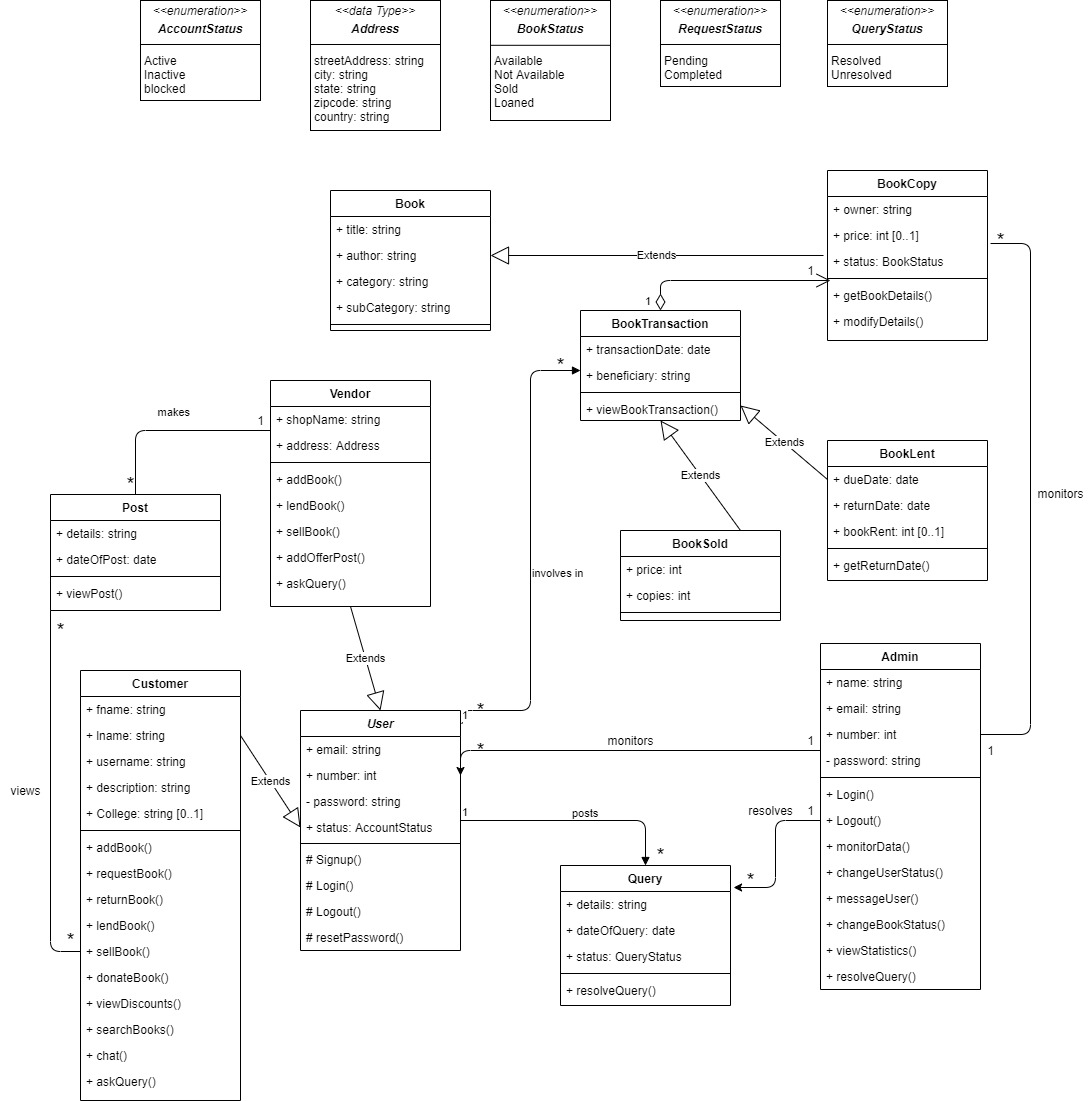
\includegraphics[scale=0.22]{Class Diagram.jpg}
%     \caption{Class Diagram}
%     \label{fig:my_label}
% \end{figure}
% 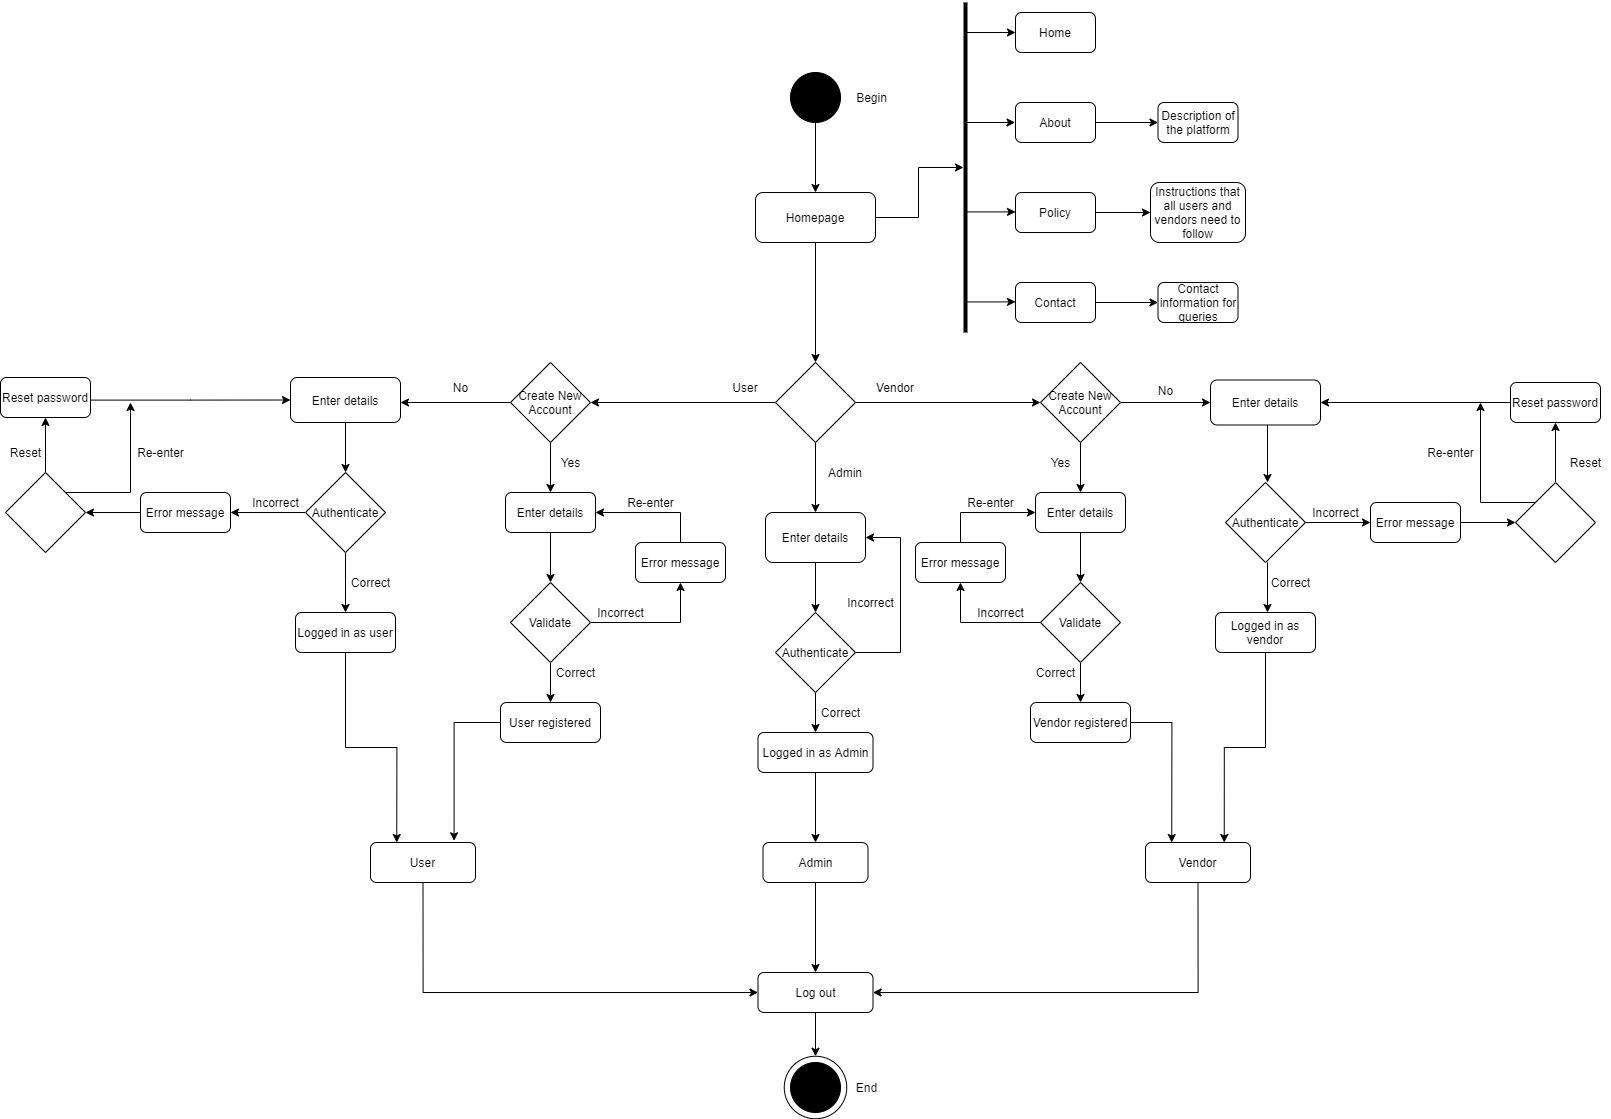
\includegraphics[scale=0.18, width=\linewidth,frame]{Activity Diagram-Main.jpg}
% 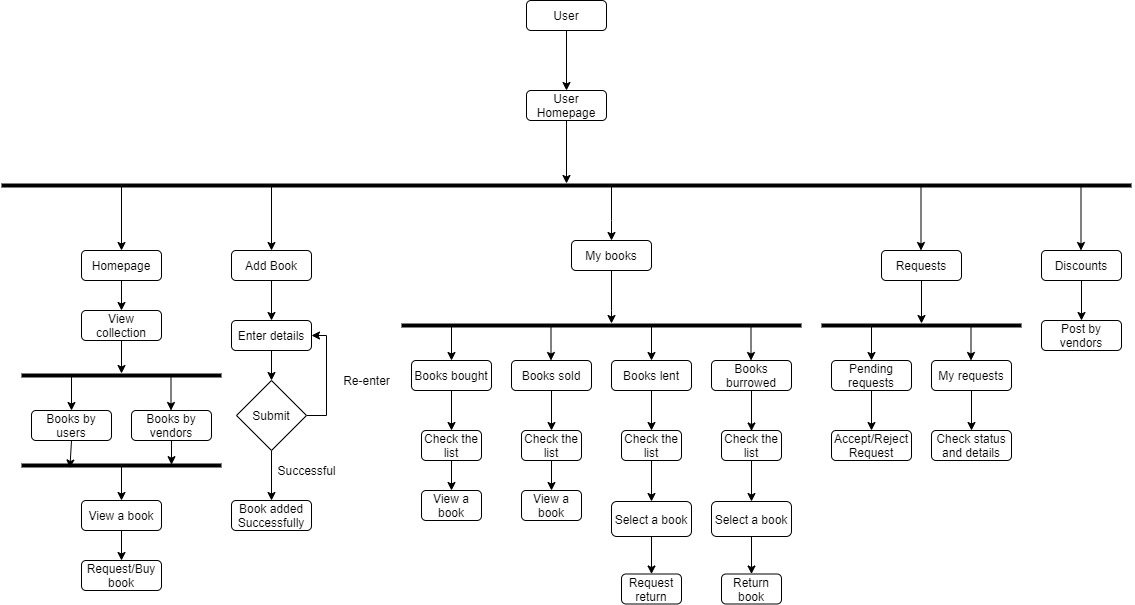
\includegraphics[scale=0.22]{Activity Diagram-User.jpg}
% 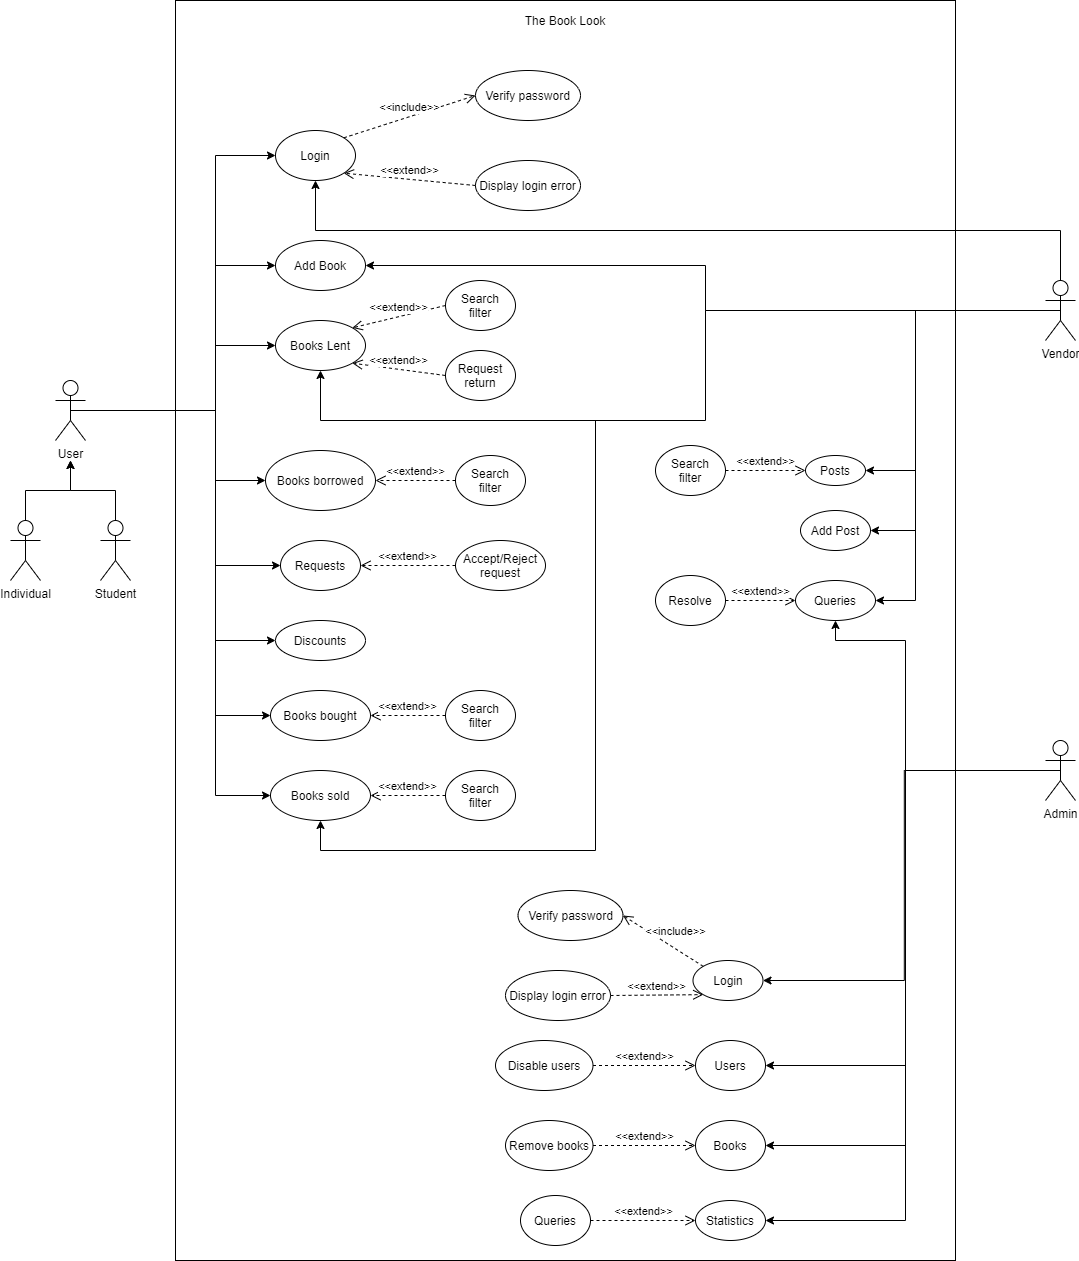
\includegraphics[scale=0.22]{Use Case Diagram.png}

\section{Introduction}
\subsection{Problem Statement and Motivation}
In today's fast flowing world, knowledge is the only constant we crave for and books are still the most relevant form of knowledge.
There are times when we want a book for a short duration but are not sure where to find it and knocking every door isn't the most feasible way out. Also the naive practice of exchanging books makes it a bit problematic to track and keep records of the books you have borrowed or lent.

The motivation behind this whole idea is to share resources and exchange knowledge in form of books with the entire community. This platform will help people to search for the book they want, borrow it or buy it according to their convenience as well as sell it or lend it. It will reduce the hassle of spending a lot of time over finding a book offline.

\subsection{Objectives}
The system consists of three modules, User, Vendor and Admin. The main objectives were to keep the system user friendly, simple and easy to use.

A user must be able to navigate and search through all the books uploaded by other fellow users and vendors and should be able to borrow or even buy the book of their choice. The user module also focuses on keeping track of all the requests the user receives and allows them respond to it.

Similarly the Vendor module enables the local shopkeepers to upload the book titles and its info to the system where it can be accessed by the users. The vendor module will also help them keep track of the books they have sold or given on rent.

The Admin module helps the designated person oversee the activities performed and see some of the statistics related to the system. 
\subsection{Our Approach}
The initial step was to understand the problem statement and then gather the requirements of the system. Afterwards we finalized the functionalities after discussing with our mentor. To get a clearer picture of the system we made the UI Design of the system and also created various UML diagrams. After studying the requirements of the system in depth, we looked for various tools and technologies to develop the system. After that during the development phase we started developing the system, module wise and kept on adding the functionalities that we had pre-decided. After the system was developed we tested it and improvised according to the feedback received.

% \subsection{Maintaining the Integrity of the Specifications}

% The IEEEtran class file is used to format your paper and style the text. All margins,
% column widths, line spaces, and text fonts are prescribed; please do not
% alter them. You may note peculiarities. For example, the head margin
% measures proportionately more than is customary. This measurement
% and others are deliberate, using specifications that anticipate your paper
% as one part of the entire proceedings, and not as an independent document.
% Please do not revise any of the current designations.

\section{User Stories}
\label{section:userstories}
User Stories are a crucial part of any software development process. They help us realise the needs of various stakeholders of the system. The user stories of our system are presented below.
\subsection{User}
\begin{itemize}
    \item As a user, I want to upload the title of the book so that other users can see my book.
\item As a user, I want to add a category for my book so that it can be easily found.
\item As a user, I want to add the number of copies of the book I have so that more people can borrow/buy it.
\item As a user, I want to add a price for the book so that I can sell it.
\item As a user, I want a search feature so that I don’t have to scroll through the entire list.
\item As a user, I want a request book feature so that I can borrow that book.
\item As a user, I want a request return feature so that I can get my lent book back.
\item As a user, I want to see my requests so that I can keep track of the requests that I have made to other users and vendors.
\item As a user, I want to see pending requests so that I can accept/reject those requests.
\item As a user, I want to see completed requests so that I can keep records of the requests that I have completed.
\item As a user, I want to lend a book so that others can also read it.
\item As a user, I want to buy a book so that I can read it.
\item As a user, I want to sell my book as I no longer need it.
\item As a user, I want to donate a book so that the needy could be helped.
\item As a user, I want to see the list of lent books so that I can oversee my books.
\item As a user, I want to see the list of borrowed books so that I can keep track of their due dates.
\item As a user, I want a chat feature so that I can interact with other book enthusiasts.
\item As a user, I want to add my bio so that others can view my interests.
\item As a user, I want to see the list of posts by vendors so that I am updated about their new offers and discounts.
\end{itemize}
\subsection{Vendor}
\begin{itemize}
    \item As a vendor, I want to upload the title of the book so that all the users can see my book.
\item As a vendor, I want to add a category for my book so that it can be easily found.
\item As a vendor, I want to add the number of copies of the book I have so that more people can borrow/buy it.
\item As a vendor, I want to add details about the rent of the book so that people can read it for a particular duration by paying money.
\item As a vendor, I want to add a price for the book so that I can sell it.
\item As a vendor, I want to see pending requests so that I can accept/reject those requests.
\item As a vendor, I want to see completed requests so that I can keep records of the requests that I have completed.
\item As a vendor, I want to put up a post on the system so that users can be informed about any offers or discounts on books.
\item As a vendor, I want to update the delivery option about various books so that customers can avail this facility.
\end{itemize}
\subsection{Admin}
\begin{itemize}
    \item As an admin, I want to monitor the activities of users like enabling/disabling books so that no inappropriate book is uploaded by a user/vendor.
\item As an admin, I want to do user control i.e. enabling/disabling of accounts so that I can block the users who are not adhering to the guidelines.
\item As an admin, I want to see statistics of the system by queries so that I can get an idea about the various books which are in demand, the number of users using the system, etc.
\item As an admin, I want a feature to enable/disable sell functionality for DA-IICT students so that students can freely exchange books among themselves.

\end{itemize}


\section{UML Diagrams}
\subsection{Class Diagram}
Class Diagram describes the structure of the system and the relation between different classes of the system. The interactions between different classes of the system are also captured. The class diagram of our system is shown in figure \ref{fig:classdiagram}. 
\begin{figure}[h]
     \centering
     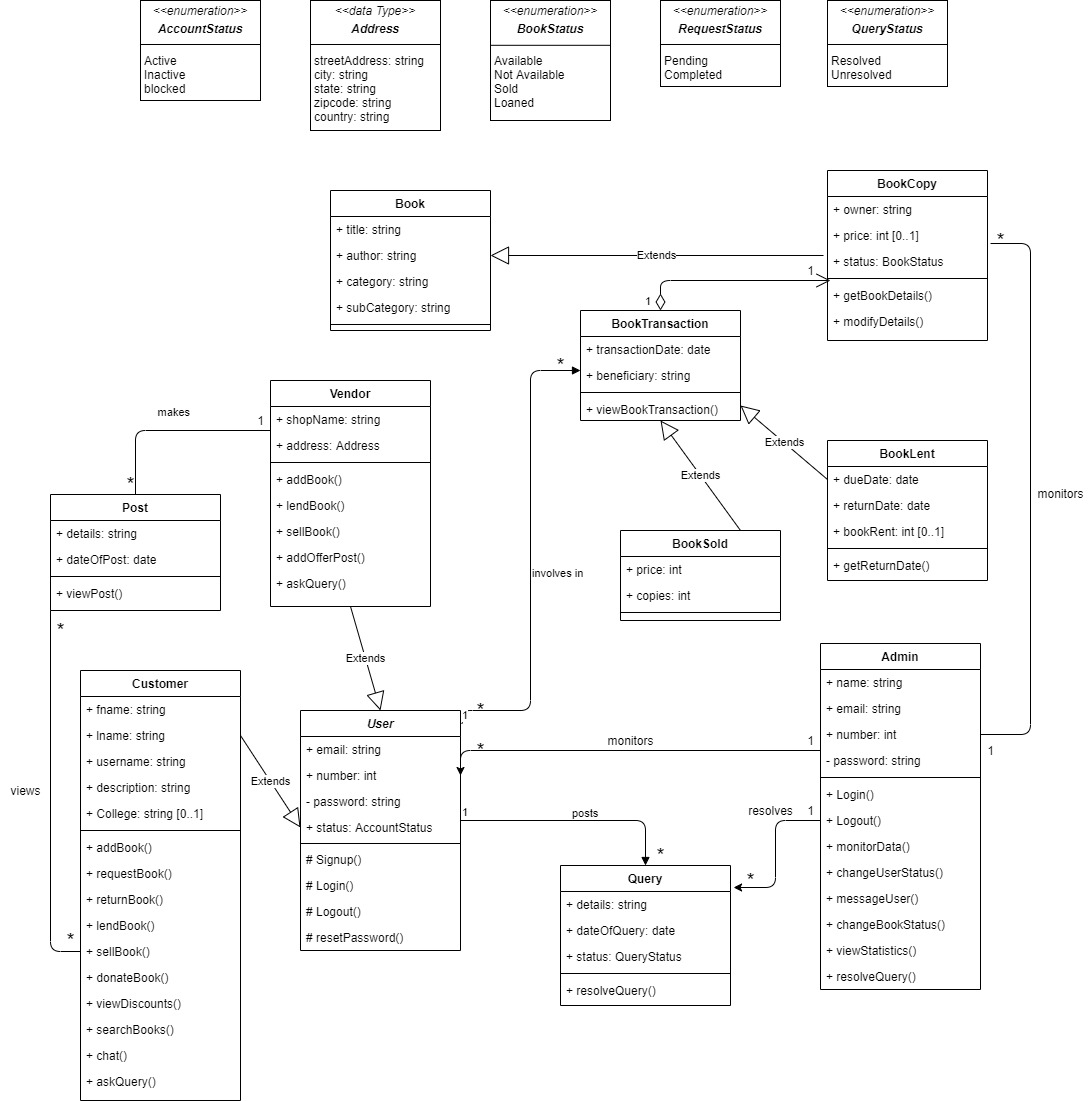
\includegraphics[scale=0.20,margin=2,frame]{Class Diagram.jpg}
     \caption{Class Diagram}
     \label{fig:classdiagram}
 \end{figure}
\subsection{Use Case Diagram}
The Use Case diagram of the system is shown in figure \ref{fig:usecasediagram}. It summarises the relationship between different actors, use cases and the system. The actors of the our system are \emph{users}, \emph{vendors} and \emph{admin}. The diagram shows the interaction of the actors with the system.
\begin{figure}[h]
     \centering
     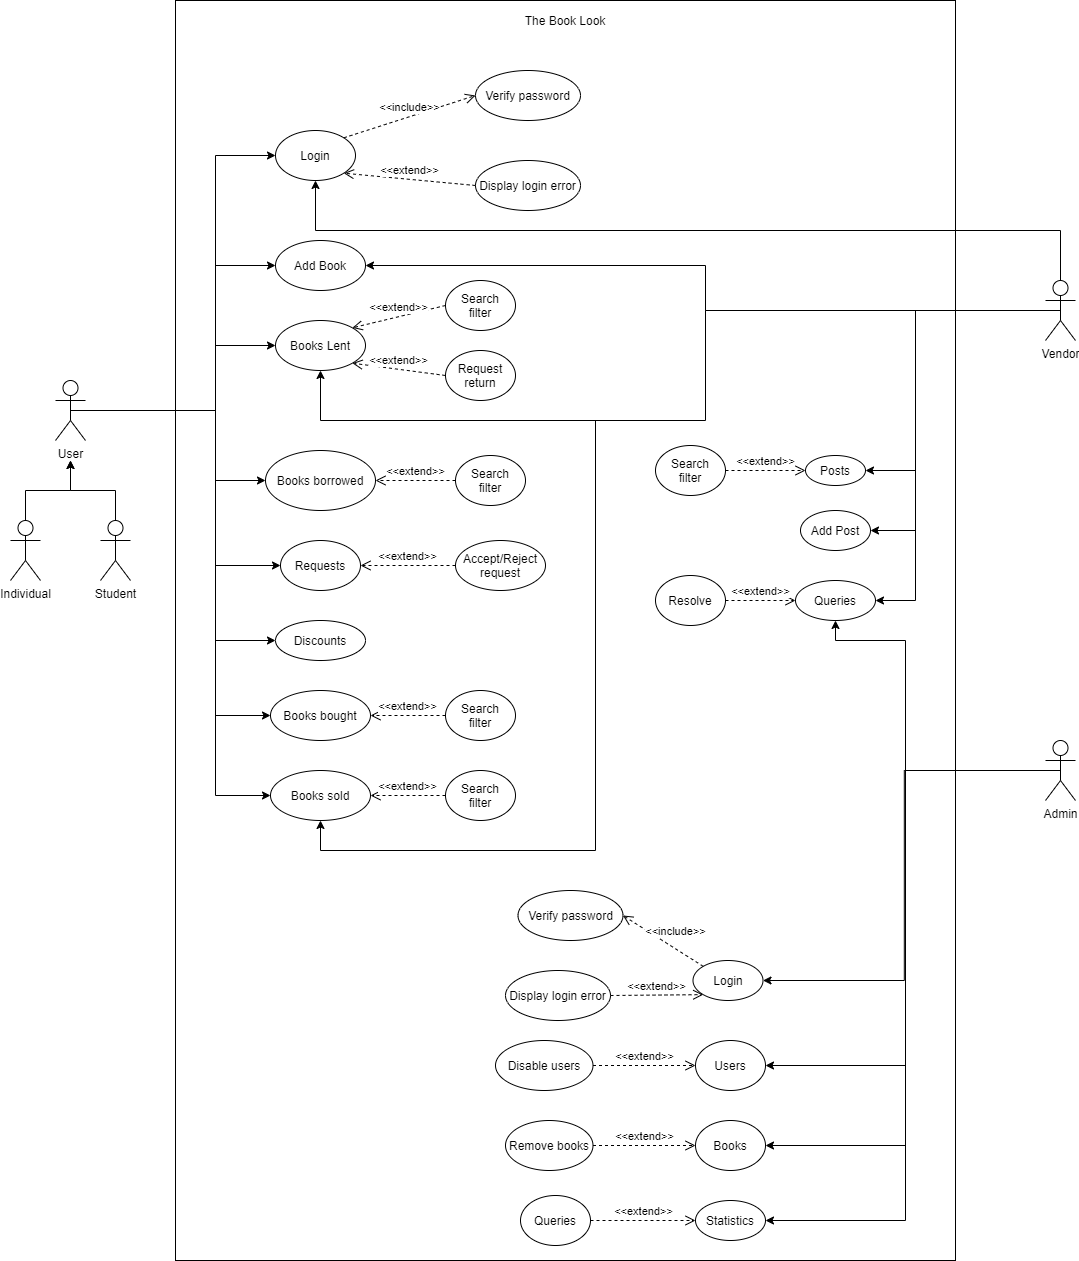
\includegraphics[scale=0.18,margin=2,frame]{Use Case Diagram.png}
     \caption{Use Case Diagram}
     \label{fig:usecasediagram}
 \end{figure}
\subsection{Activity Diagram}
The Activity Diagram of the system depicts the flow of control from the starting point to the finishing point with various conditional paths in between. It portrays the step wise activities and functionalities of the system. The Activity Diagram of our system is divided into four parts. 
\subsubsection{Activity Diagram - Main}
This part shows the overall flow of control of the system starting from the login to logout. The parts \emph{user}, \emph{vendor}, \emph{admin} present in this part are enlarged in other parts. Figure \ref{fig:activitydiagrammain} shows this part of the Activity Diagram.
\begin{figure}[h]
     \centering
     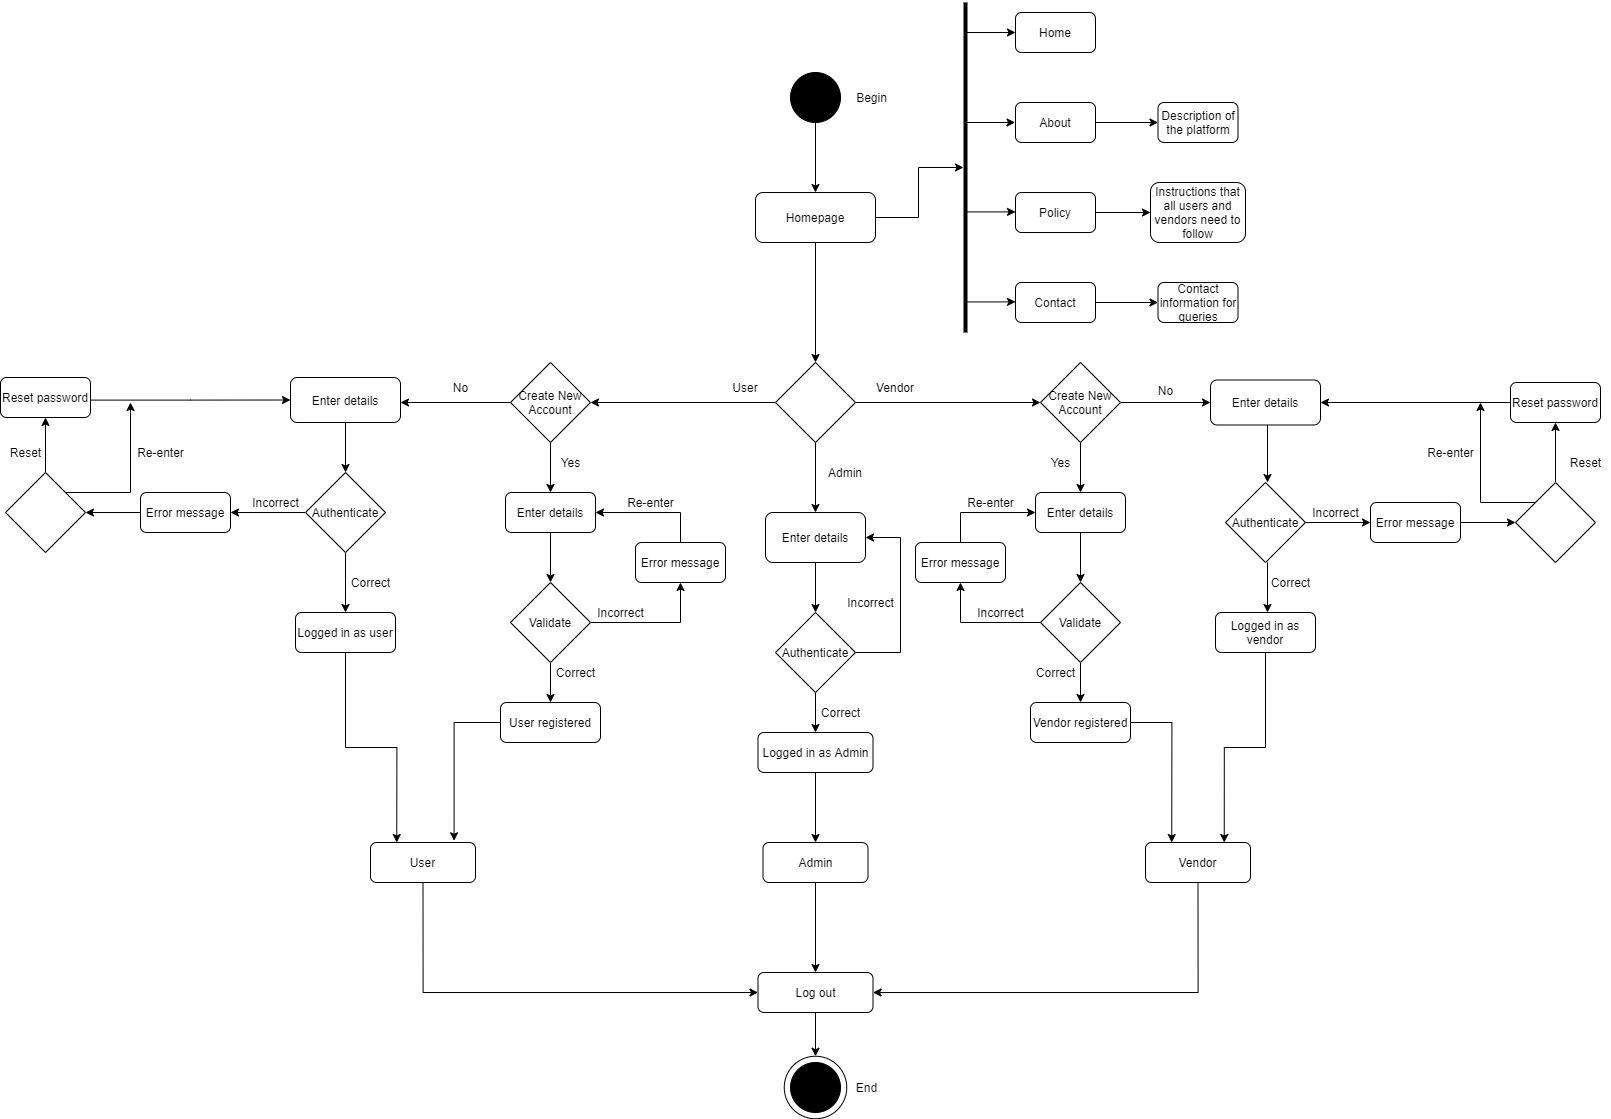
\includegraphics[scale=0.15,margin=2,frame]{Activity Diagram-Main.jpg}
     \caption{Activity Diagram - Main}
     \label{fig:activitydiagrammain}
 \end{figure}
 \subsubsection{Activity Diagram - User}
 This part shows the detailed flow of the user module. All the features available to the user as well as their flow of control in shown in figure \ref{fig:activitydiagramuser}.
 \begin{figure}[H]
     \centering
     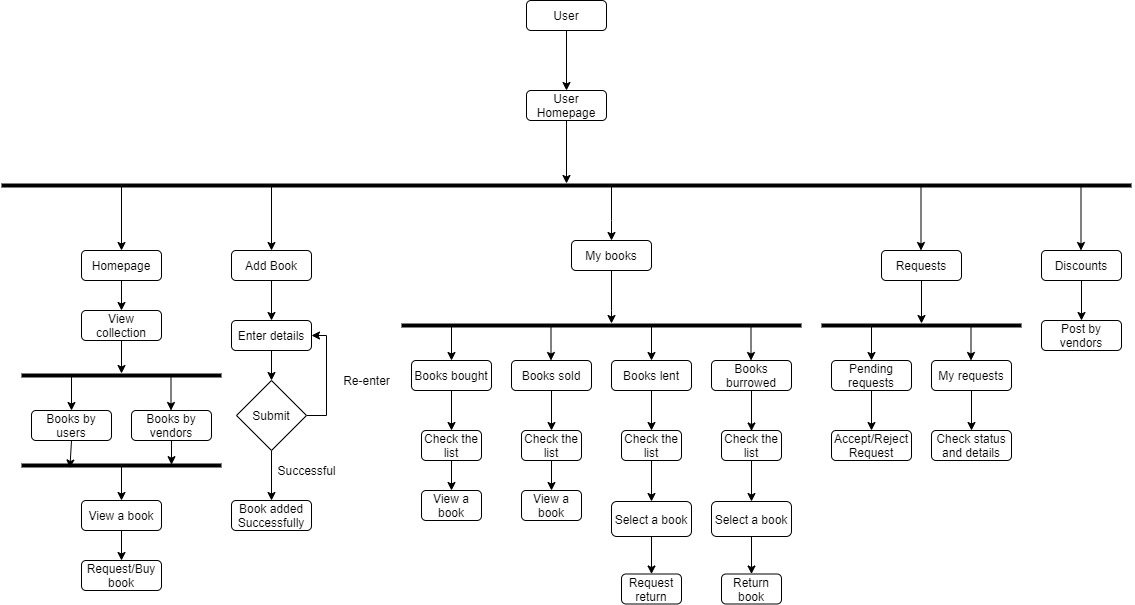
\includegraphics[scale=0.18,margin=2,frame]{Activity Diagram-User.jpg}
     \caption{Activity Diagram - User}
     \label{fig:activitydiagramuser}
 \end{figure}
 \subsubsection{Activity Diagram - Vendor}
 This part shows the detailed flow of the vendor module. As shown in figure \ref{fig:activitydiagramvendor}, this part depicts the step wise activities of the vendor module.
 \begin{figure}[H]
     \centering
     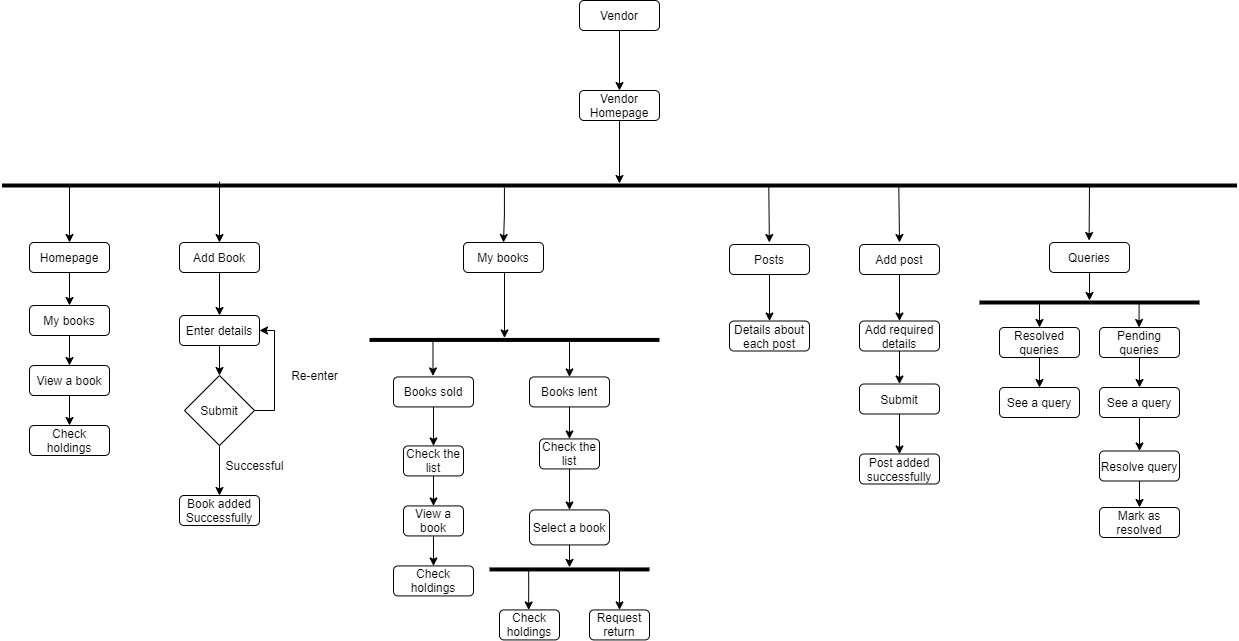
\includegraphics[scale=0.18,margin=2,frame]{Activity Diagram-Vendor.jpg}
     \caption{Activity Diagram - Vendor}
     \label{fig:activitydiagramvendor}
 \end{figure}
 \subsubsection{Activity Diagram - Admin}
 This part corresponds to the Admin module. All the actions and their flow are captured in this part as shown in figure \ref{fig:activitydiagramadmin}.
 \begin{figure}[h]
     \centering
     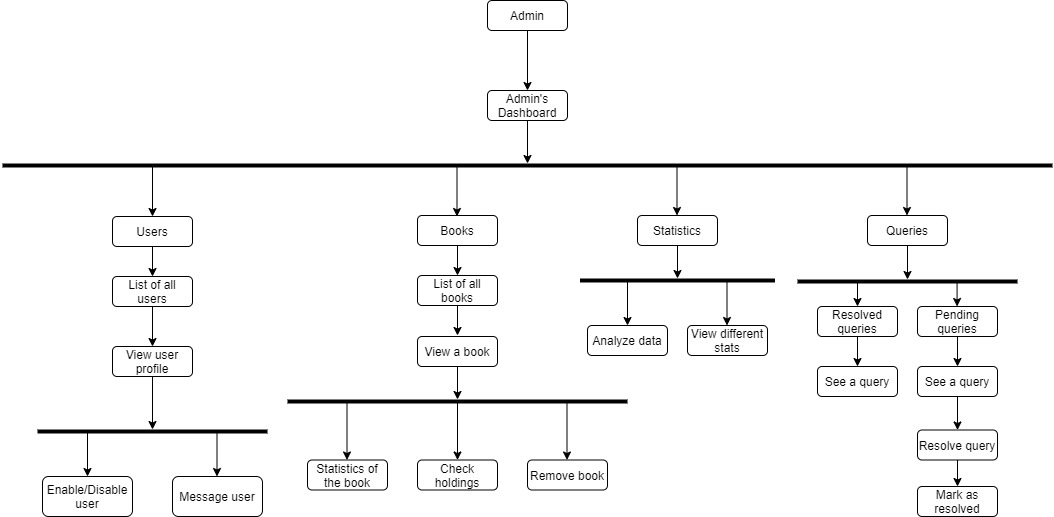
\includegraphics[scale=0.18,margin=2,frame]{Activity Diagram-Admin.jpg}
     \caption{Activity Diagram - Admin}
     \label{fig:activitydiagramadmin}
 \end{figure}
\subsection{Sequence Diagram}
Sequence Diagram captures the interaction of various systems with each other and captures how different elements interact over time. The vertical axis displays time while the horizontal axis shows the elements involved in the interaction. The Sequence Diagrams of the system are shown in figure \ref{fig:sequencediagramaddbook} and \ref{fig:sequencediagrambuysell}.
\begin{figure}[H]
     \centering
     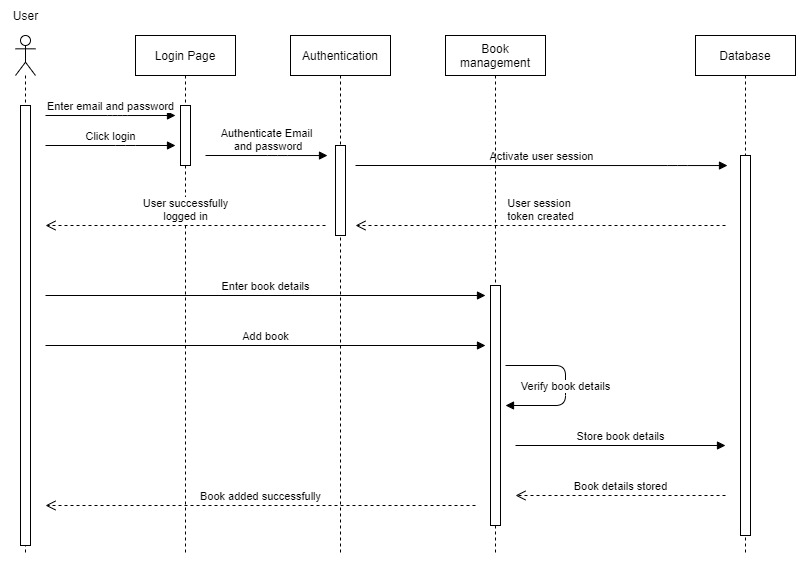
\includegraphics[scale=0.20,margin=2,frame]{Sequence Diagram-Add Book.jpg}
     \caption{Sequence Diagram - Add Book}
     \label{fig:sequencediagramaddbook}
 \end{figure}
 \begin{figure}[H]
     \centering
     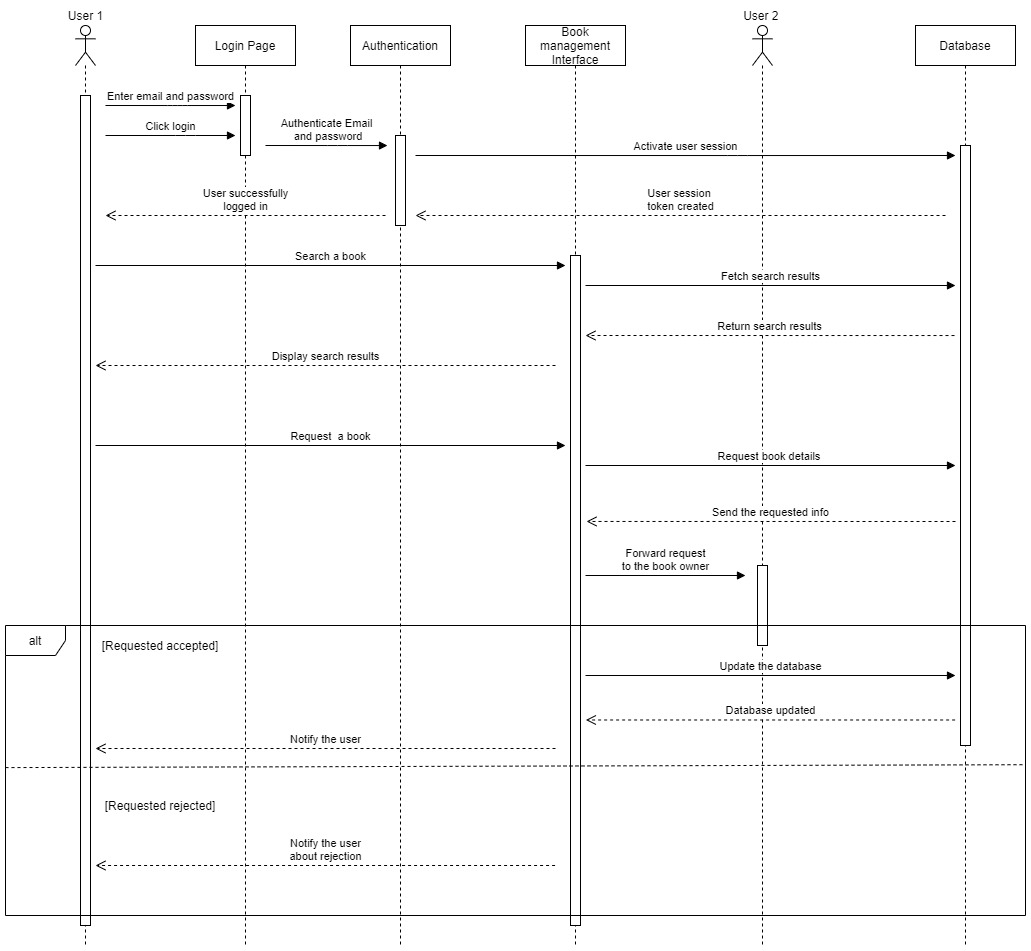
\includegraphics[scale=0.20,margin=2,frame]{Sequence Diagram-Buy_Sell.jpg}
     \caption{Sequence Diagram - Buy/Sell}
     \label{fig:sequencediagrambuysell}
 \end{figure}

\section{Functionalities of the System}
The user stories presented in Section \ref{section:userstories} are elaborated here. This section provides a detailed description of all the functionalities of the system.
\subsection{Signup/Login}

\subsubsection{User module}
A user will need to register himself/herself on the Web Application by signing up before using the system. A user will need to fill in the details like first name, last name, college, email and password. 
\begin{figure}[h]
     \centering
     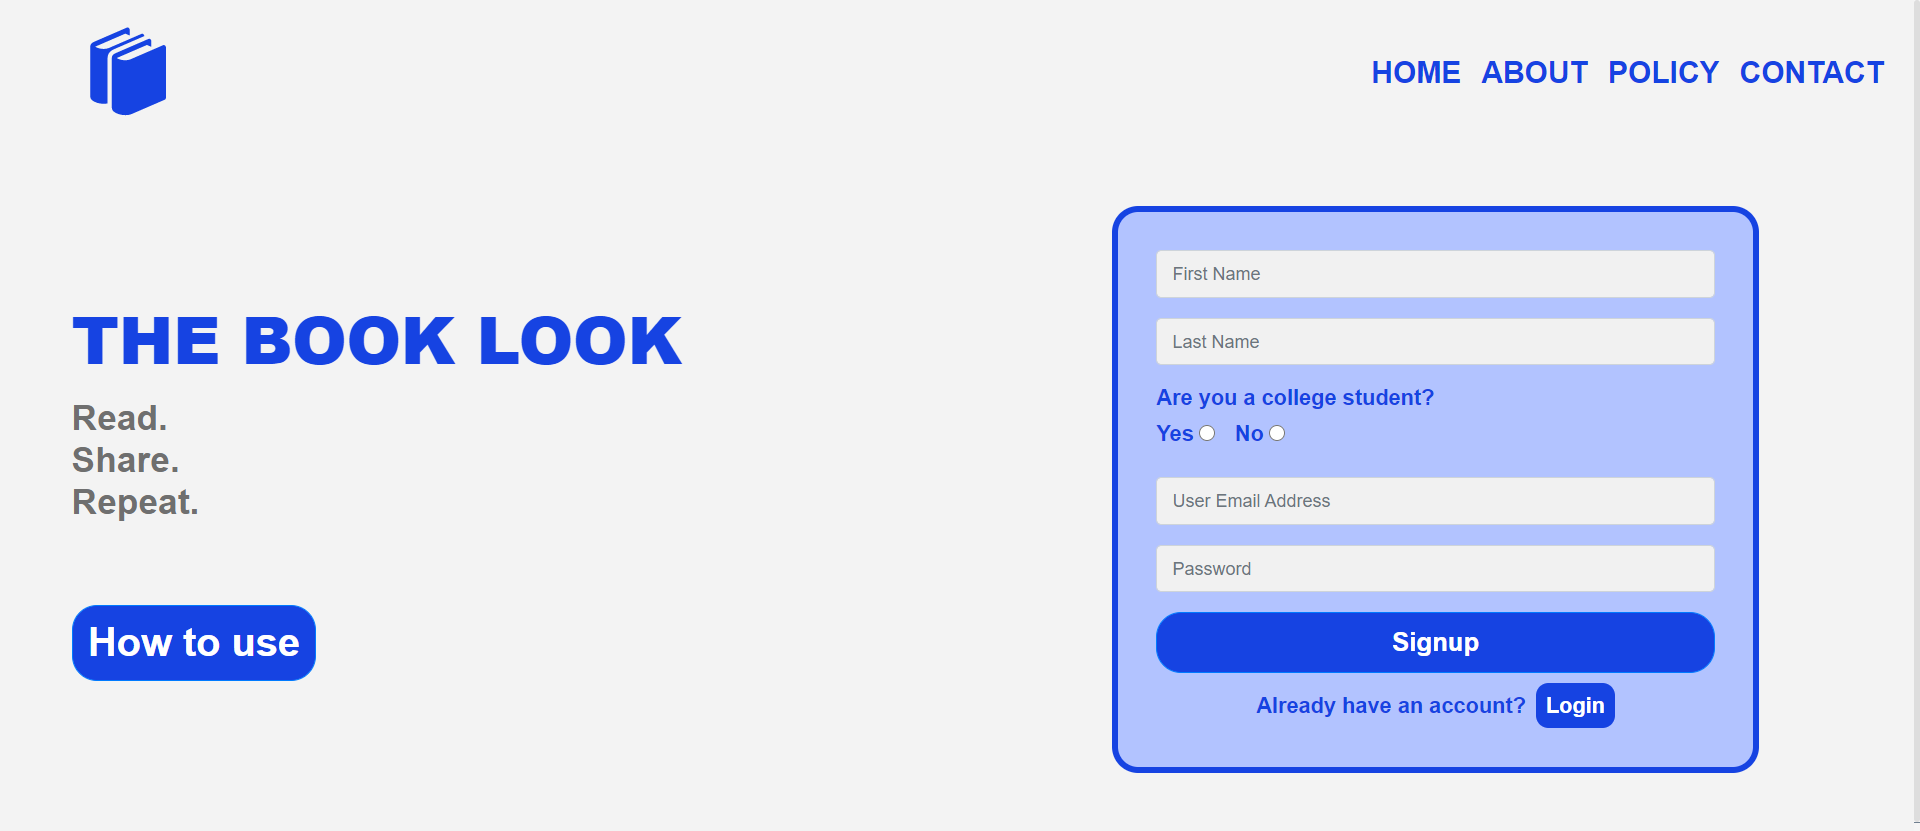
\includegraphics[scale=0.20,margin=2,frame]{signup.PNG}
     \caption{User Signup}
     \label{fig:signup}
 \end{figure}
After signing up, a verification mail will be sent to the user on their email id and the user will need to verify their email by clicking on the link present in the email.
\begin{figure}[h]
     \centering
     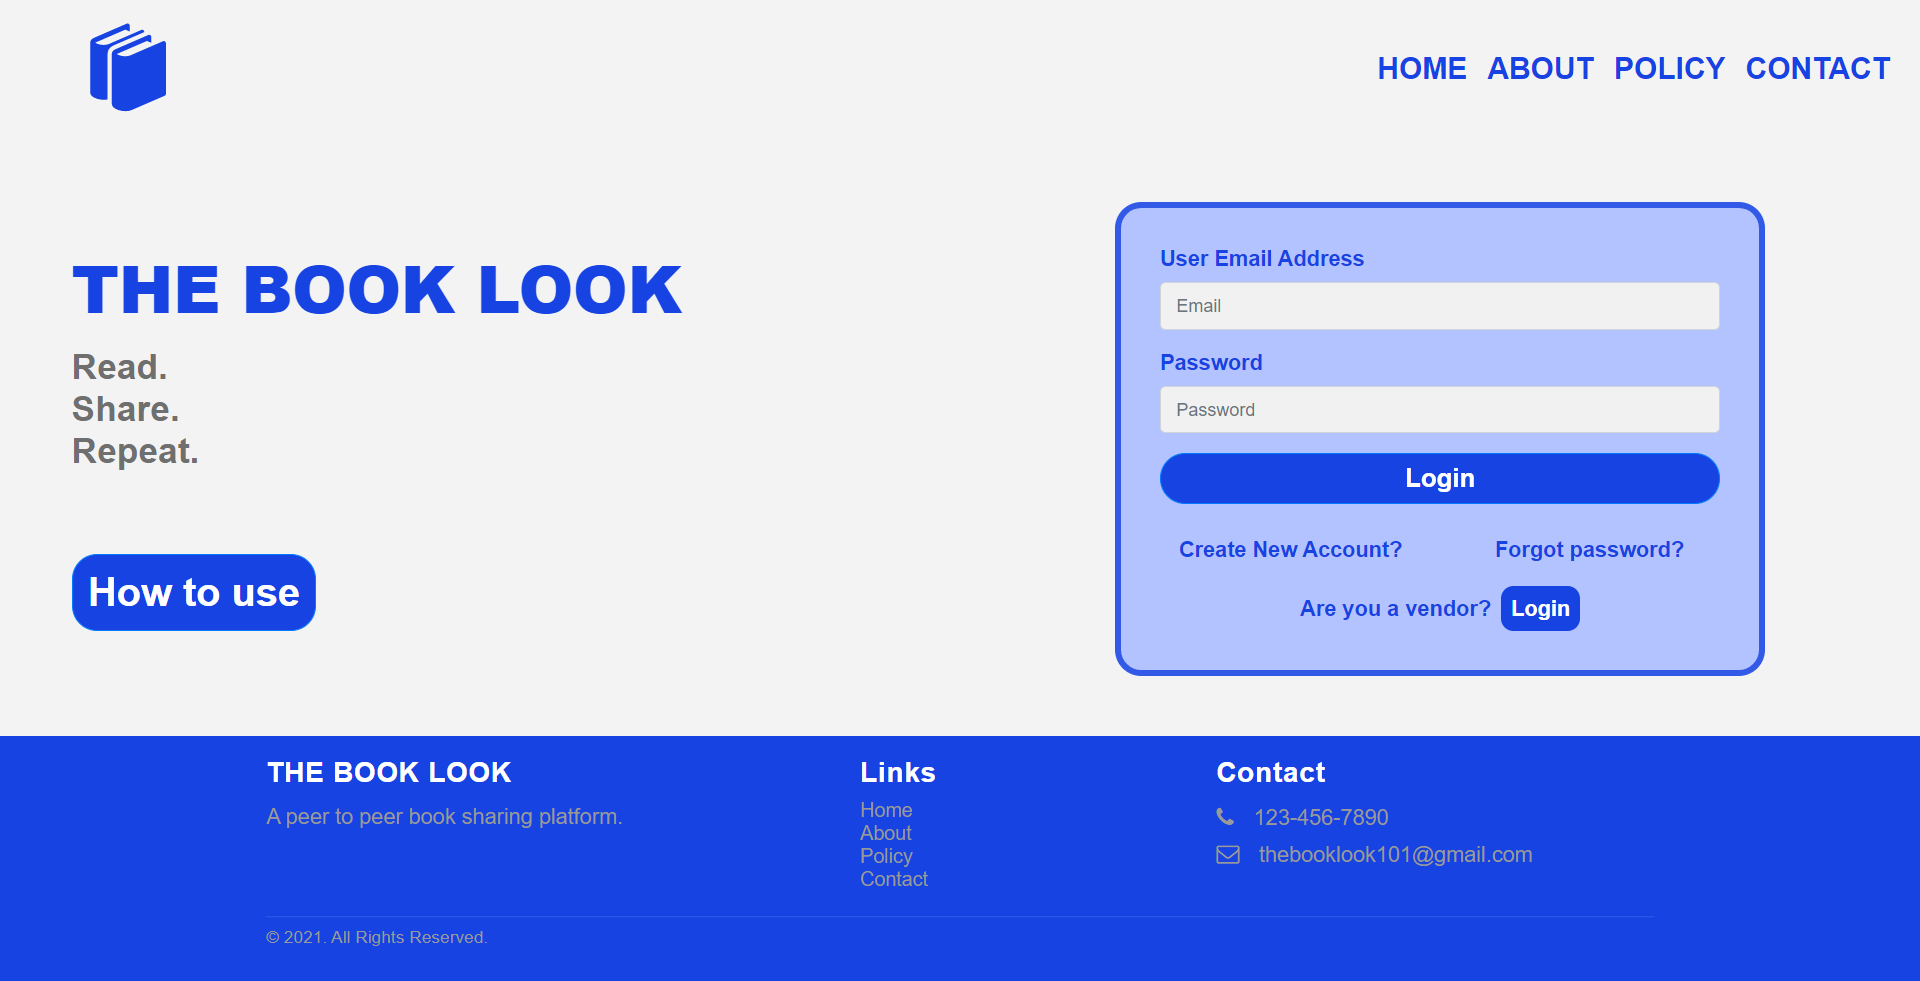
\includegraphics[scale=0.20,margin=2,frame]{login.PNG}
     \caption{User Login}
     \label{fig:login}
 \end{figure}
Without verification, the user won't be allowed to login into the system. After successful verification a user can either login to the system through the link provided in the email or by logging in through the Login page of the system shown in figure \ref{fig:login}.
\vspace{3mm}
\subsubsection{Vendor module}
A vendor will need to follow a similar process to register his/her shop on the system. While signing up, other than the detail's mentioned in the user module, the vendor will also have to provide the name of his/her shop. And after successful verification the vendor will be able to log in into the system through vendor's login page.
\vspace{3mm}
\subsubsection{Admin module}
The Admin module does not contain the sign up part. The Admin will be given a predefined set of credentials through which he/she will be able to log in into the system.

\subsection{Forgot Password}
The user module as well as the vendor module contains the feature of forgot password that enables them to change their password. 
\begin{figure}[h]
     \centering
     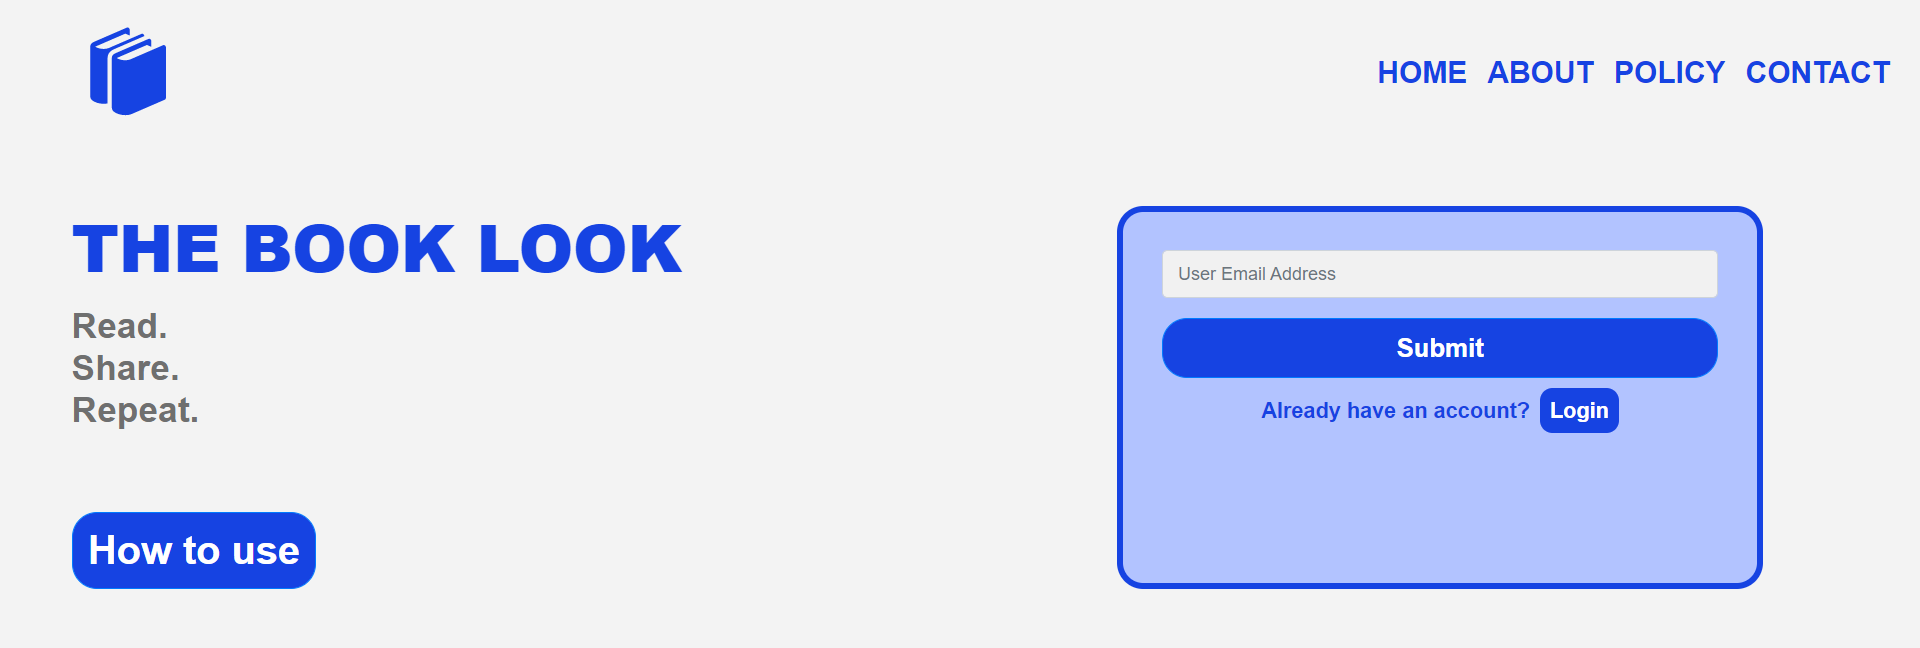
\includegraphics[scale=0.20,margin=2,frame]{forgotpassword.PNG}
     \caption{Forgot Password}
     \label{fig:forgotpassword}
 \end{figure}
The \emph{Forgot Password} link will redirect to a new page as shown in figure \ref{fig:forgotpassword} where the user/vendor will be asked to enter their email id. After hitting submit, an email will be sent to the user/vendor which will contain the link through which they will be able to reset their password.

\subsection{Viewing the collection of books}
The books are distributed into three sub-sections as shown in figure \ref{fig:usersbooks}.
\begin{figure}[h]
     \centering
     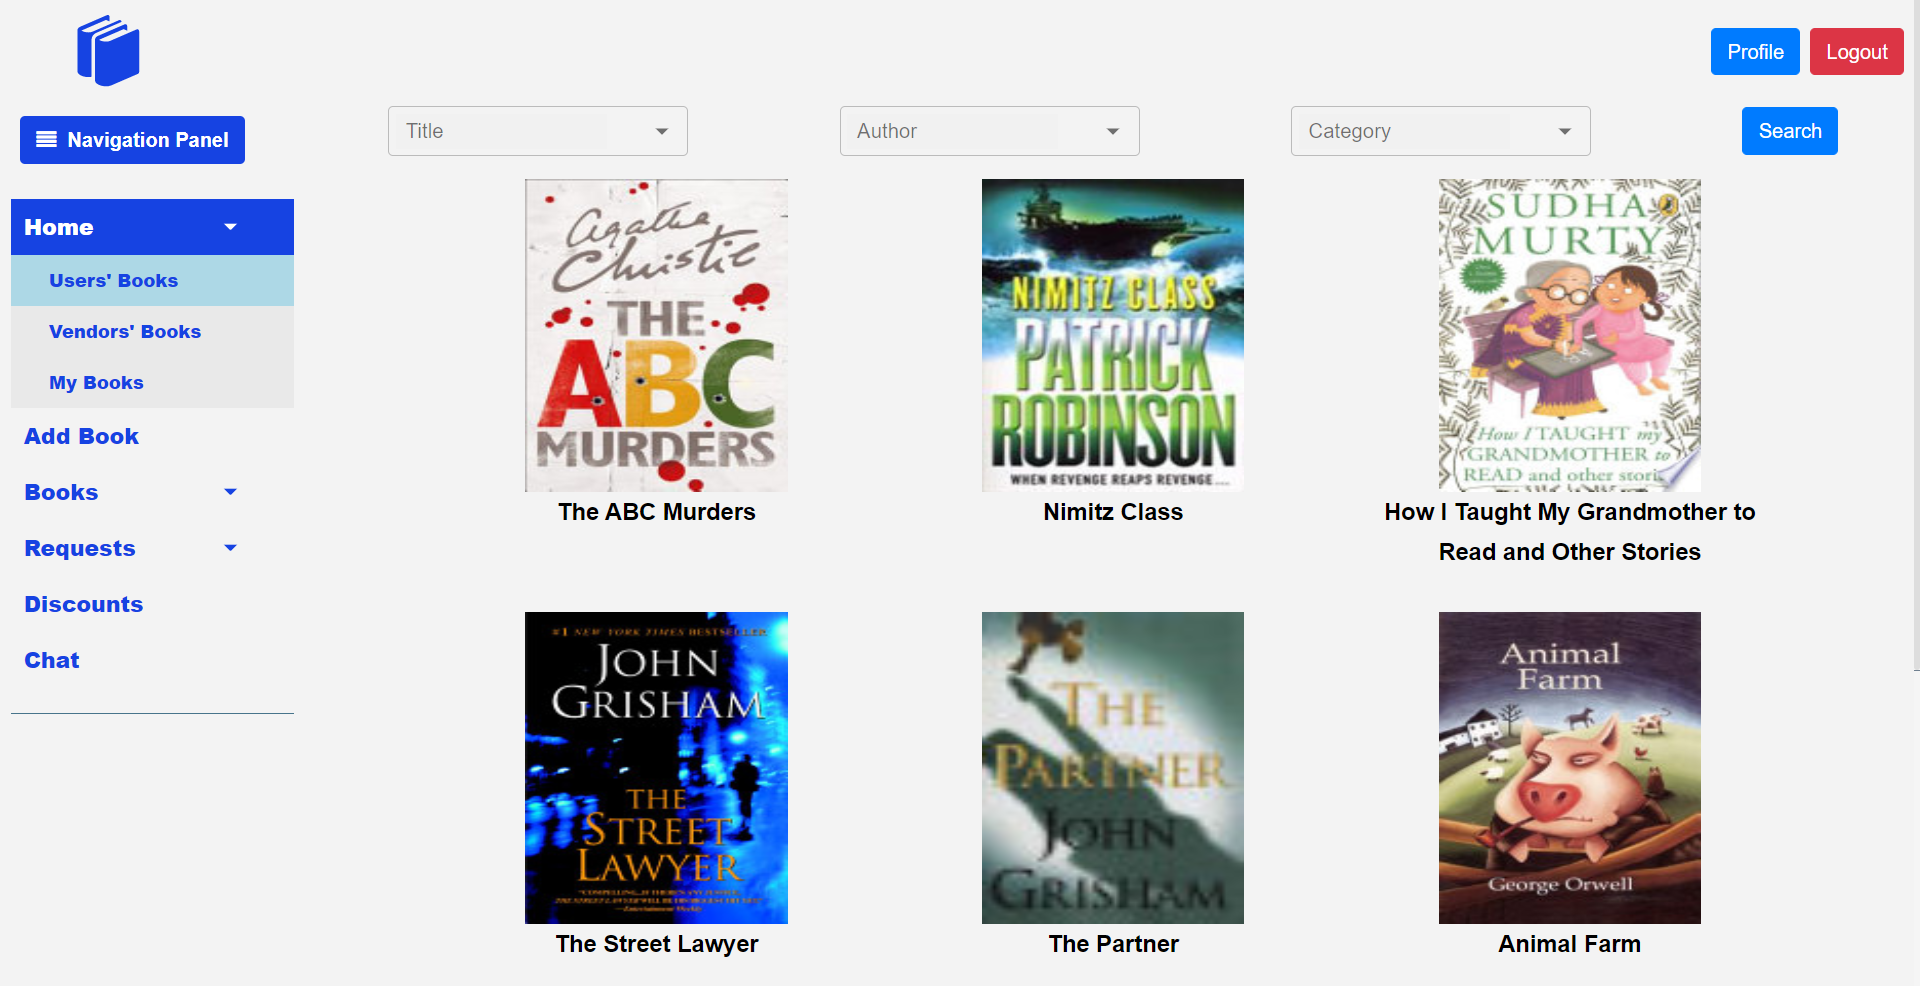
\includegraphics[scale=0.20,margin=2,frame]{usersbooks.PNG}
     \caption{Users' Books}
     \label{fig:usersbooks}
 \end{figure}
 \begin{figure}[h]
     \centering
     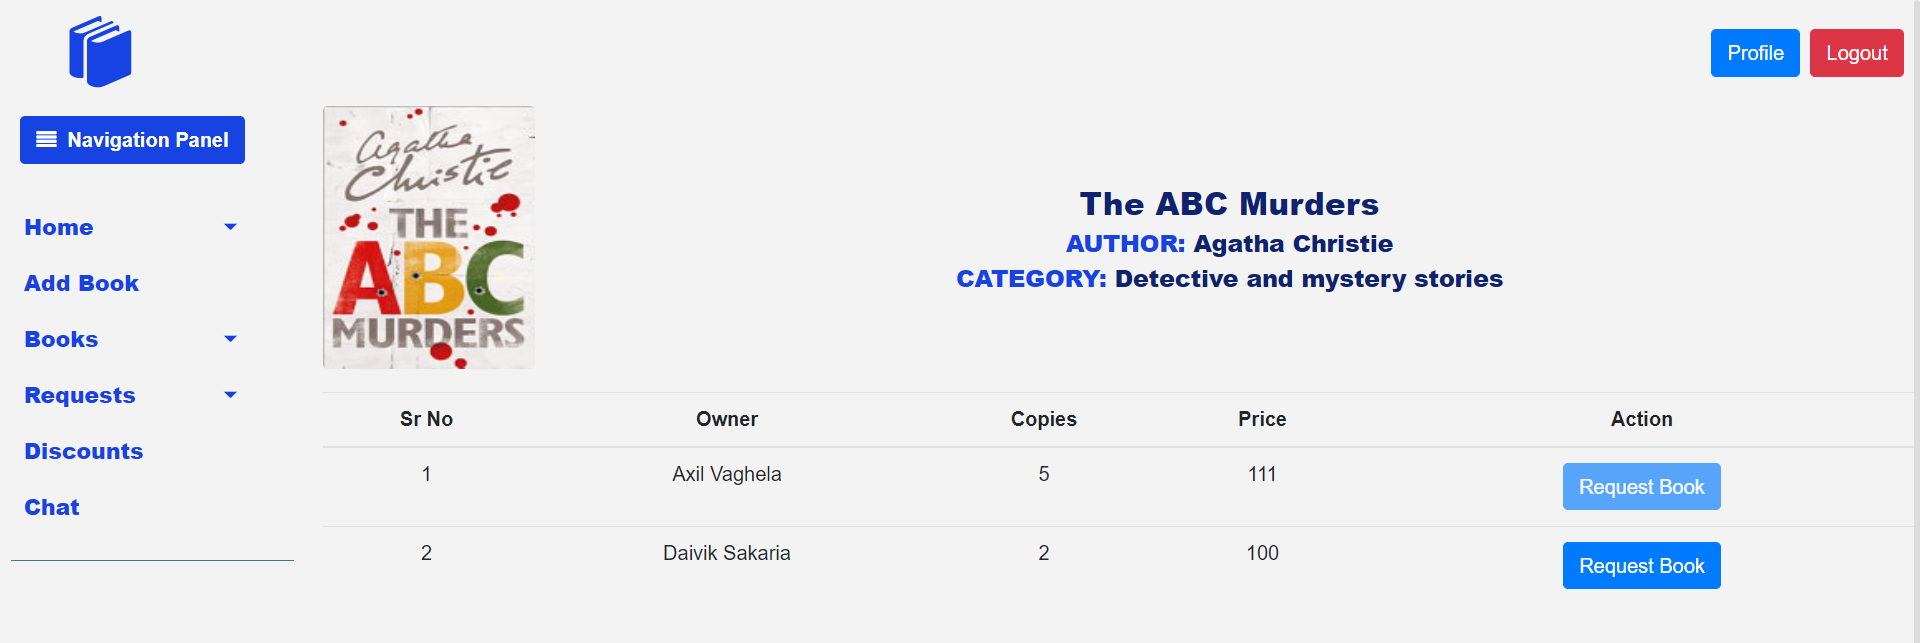
\includegraphics[scale=0.20,margin=2,frame]{individualbook.PNG}
     \caption{Individual book}
     \label{fig:individualbook}
 \end{figure}
\subsubsection{User Books}
This section contains the books uploaded by fellow users which can be bought or borrowed. 
\subsubsection{Vendor Books}
This section contains the books uploaded by vendors which can be bought or borrowed on rent basis.
\subsubsection {My Books}
This section contains the books added by the user to the system.

All three sections are present in the user module while the vendor homepage will only show the books uploaded by that particular vendor.

\subsection{Search}
The \emph{search} functionality helps the users and vendors to find a book easily while viewing the whole collection of books. There are three search filters available for it. The below figure shows an example of the search functionality.
\begin{figure}[ht]
     \centering
     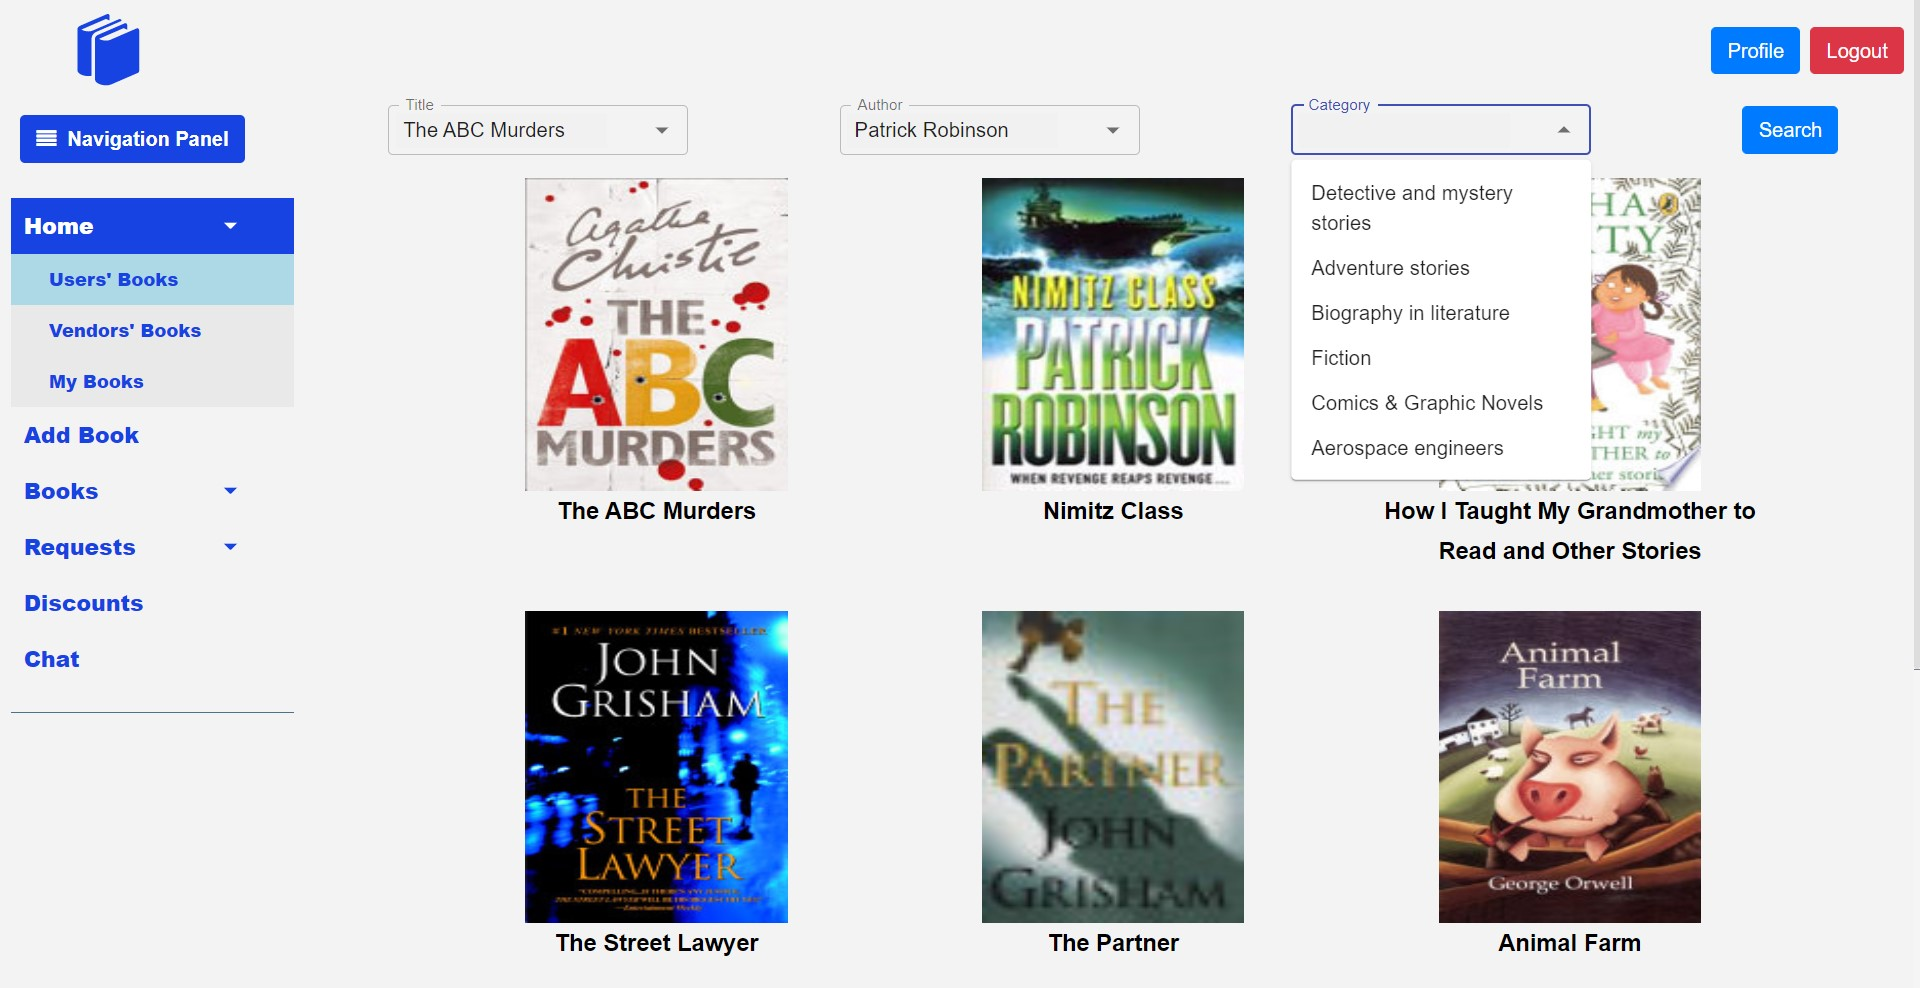
\includegraphics[scale=0.21,margin=2,frame]{search.jpg}
     \caption{Search}
     \label{fig:search}
 \end{figure}
\subsubsection{Search by title}
This filter helps the user/vendor check if a particular book is available in the collection or not. As the user/vendor will type the title name, the related titles will appear in the list and the user/vendor can select it.
\subsubsection{Search by author}
This filter helps the user/vendor find all the books by a particular author. As the user/vendor types in the field, the list of authors will be filtered and shown to them and when the \emph{search} button is clicked all the books of that particular author will be shown.
\subsubsection{Search by category}
This filter helps the user/vendor fetch all the books of a particular category. Each book as at least one category associated with it and when a particular category is chosen by a user/vendor all the books having that category will be shown.

\subsection{Add book}
To add a book to the system the user/vendor will need to provide the ISBN number of the book. Then the system will fetch the book details from the ISBN number. 
\begin{figure}[h]
     \centering
     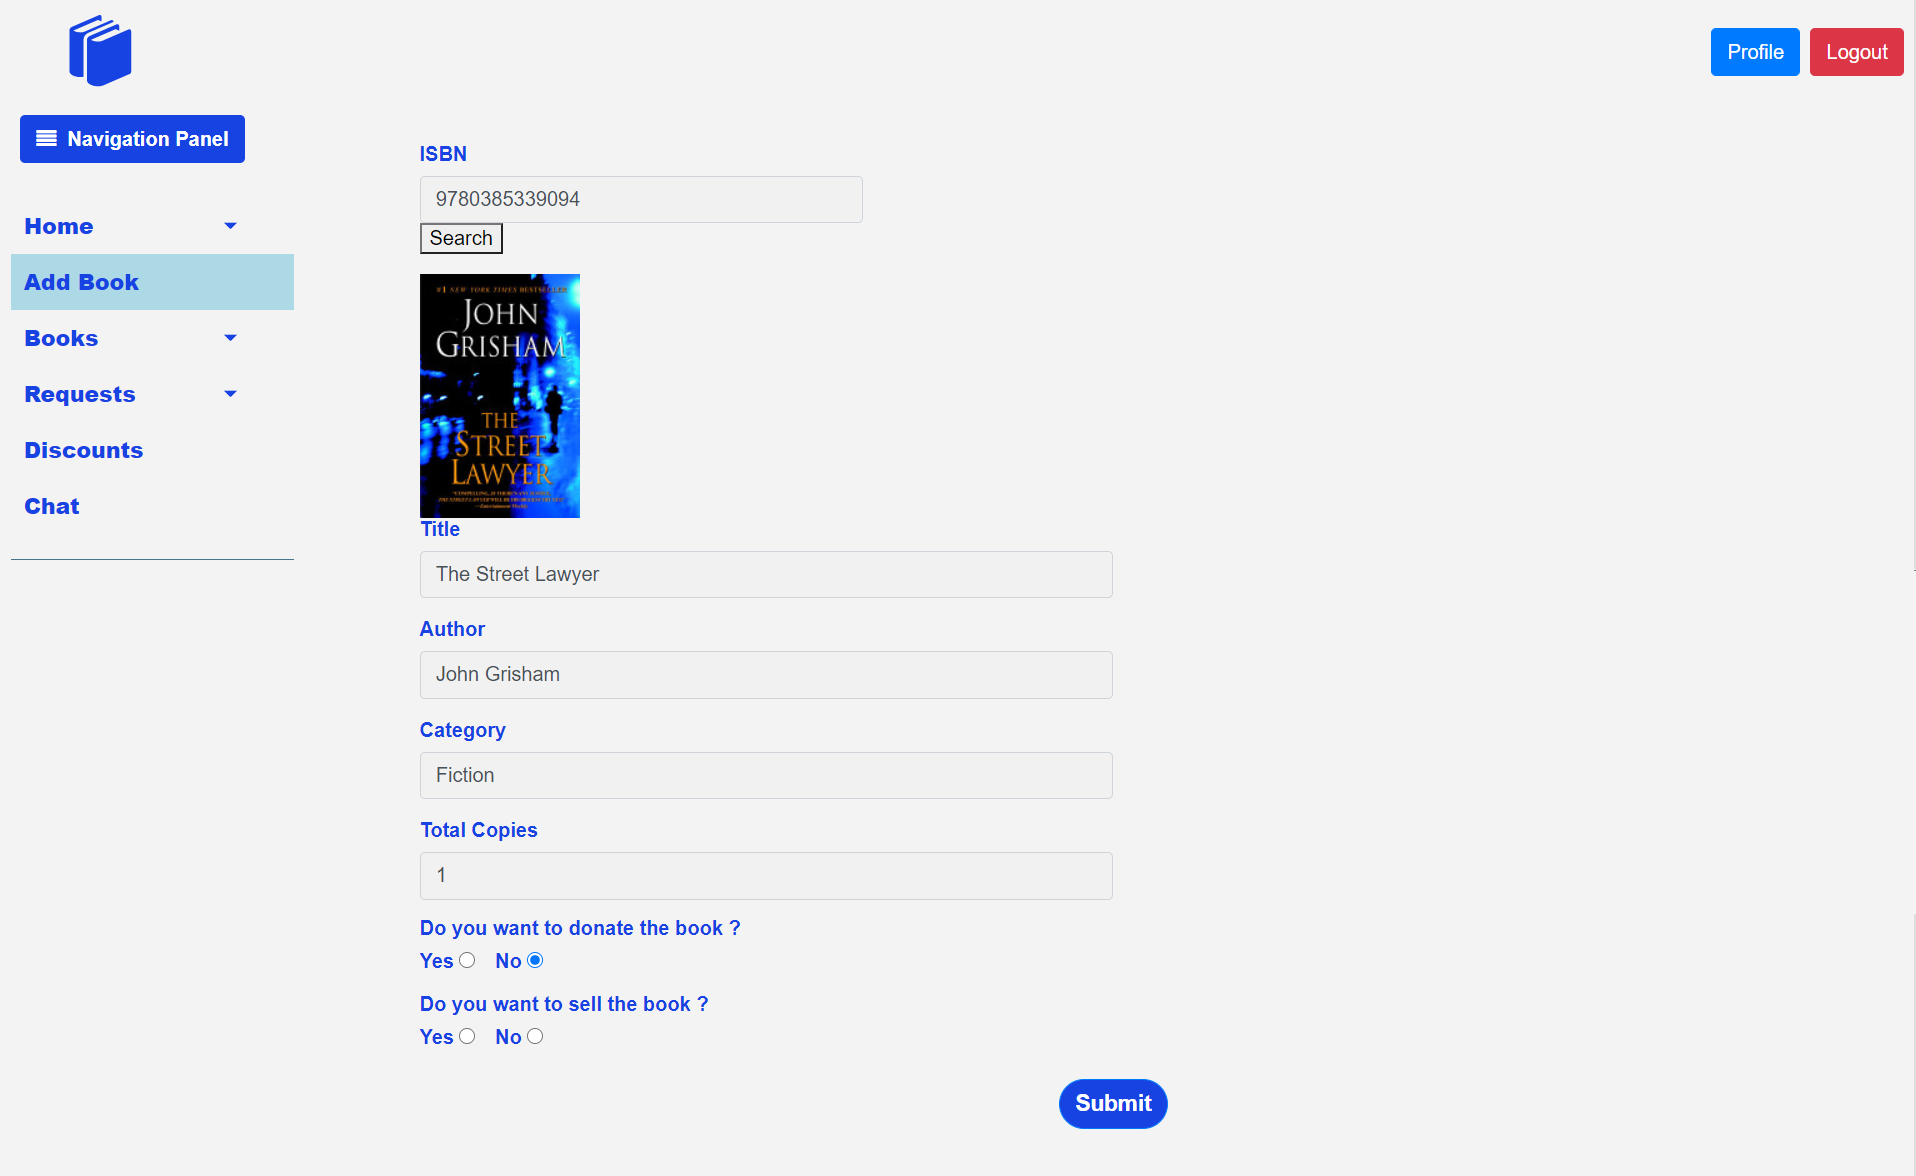
\includegraphics[scale=0.20,margin=2,frame]{addbook.png}
     \caption{Add Book}
     \label{fig:addbook}
 \end{figure}
Afterwards the user/vendor will need to fill out other details like the number of copies, price of the book or even rent in case of the vendor and then hit submit. If all the details will be appropriate then the book will be added to the system and the user/vendor will be notified.  


\subsection{Request book}
The request book feature allows a user to request to another user or vendor for a particular book. When a user clicks on a particular book in a collection it will redirect to a new page where the book details will be displayed. Along with the book details there will be a list of users and vendors who possess the book and are willing to sell or lend it. 
\begin{figure}[h]
     \centering
     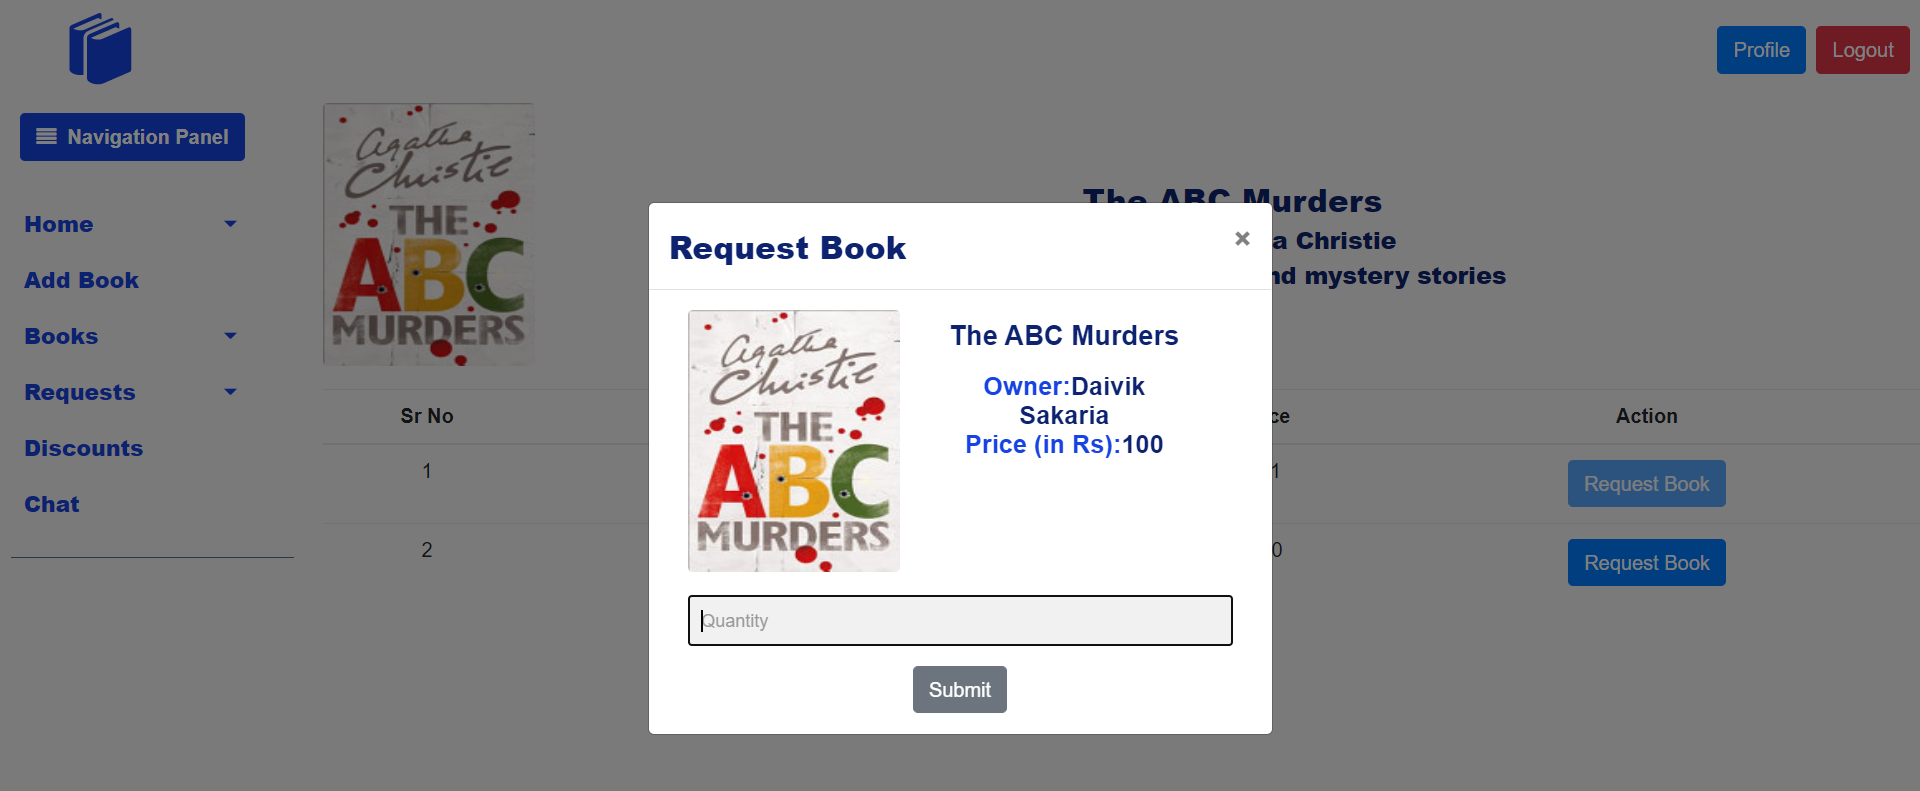
\includegraphics[scale=0.20,margin=2,frame]{requestbook.PNG}
     \caption{Request Book}
     \label{fig:requestbook}
 \end{figure}
The user can look into the list and click on the \emph{request book} button and a pop-up page will appear as shown in figure \ref{fig:requestbook}. The pop-up will display the book details as well as the details of the owner of the book. The user will then have to fill up some details like the duration for which he/she wants the book, number of copies, etc. After clicking on the submit button, the system will check the availability of the book and a request will be sent to the owner of the book with the corresponding details if available. 

\subsection{Viewing requests}
The requests are divided into three sub-sections.

\subsubsection{My requests}
This section shows the request that the user has made to other users and vendors. It shows a table containing all the requests along with details of the request like book name, date of request, copies requested, status of the request etc.
\begin{figure}[h]
     \centering
     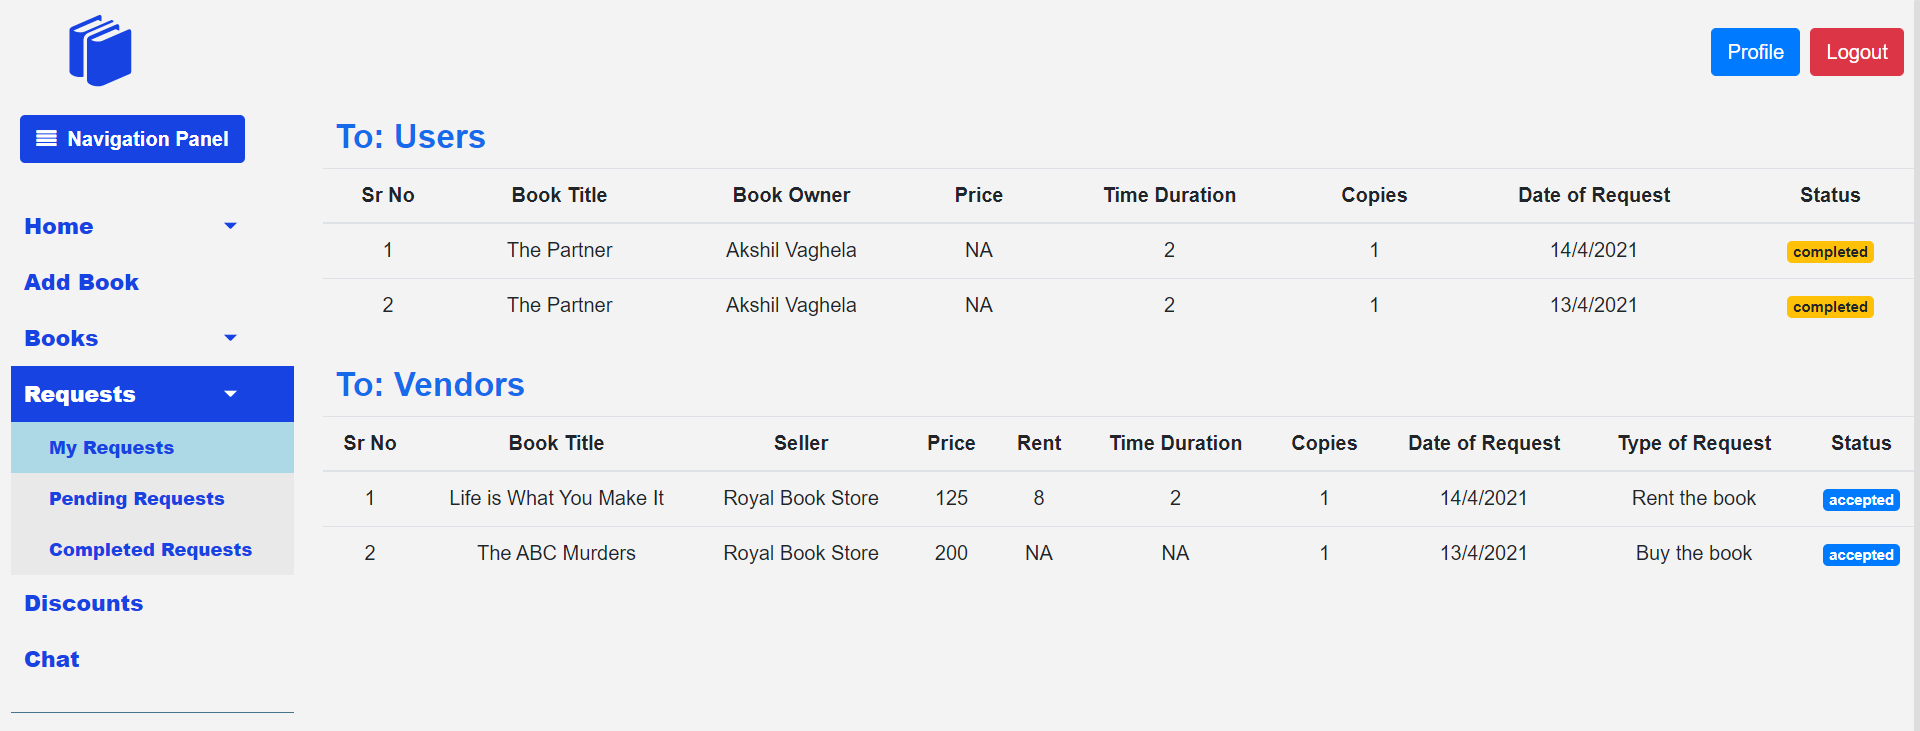
\includegraphics[scale=0.20,margin=2,frame]{myrequests.PNG}
     \caption{My requests}
     \label{fig:myrequests}
 \end{figure}

\subsubsection{Pending requests}
This section shows the requests that other users have made for a book added by the current user/vendor. The request shows the name of the requester, number of copies, duration etc. With every request there is an option for the user to \emph{Accept} or \emph{Reject} the request. As soon as the user clicks on either, the request vanishes from there and the user will be notified about the action performed.
\begin{figure}[h]
     \centering
     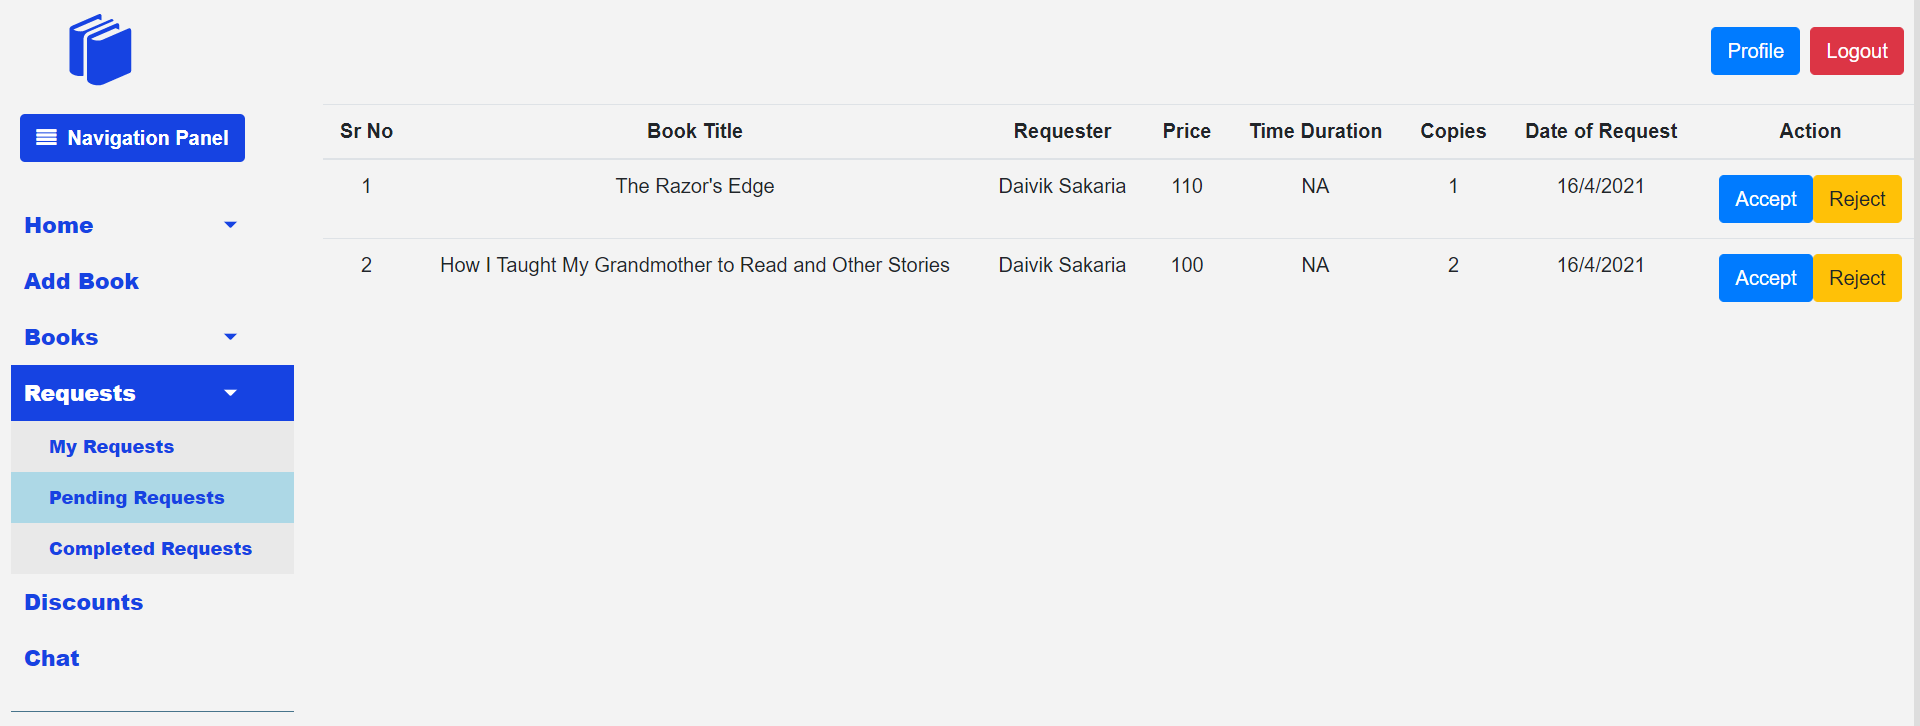
\includegraphics[scale=0.20,margin=2,frame]{pendingrequests.PNG}
     \caption{Pending Requests}
     \label{fig:pendingrequests}
 \end{figure}

\subsubsection{Completed requests}
This section shows the request that a user/vendor has completed. When a user accepts/rejects a request, that request is then moved to this section along with its corresponding status. 
\begin{figure}[h]
     \centering
     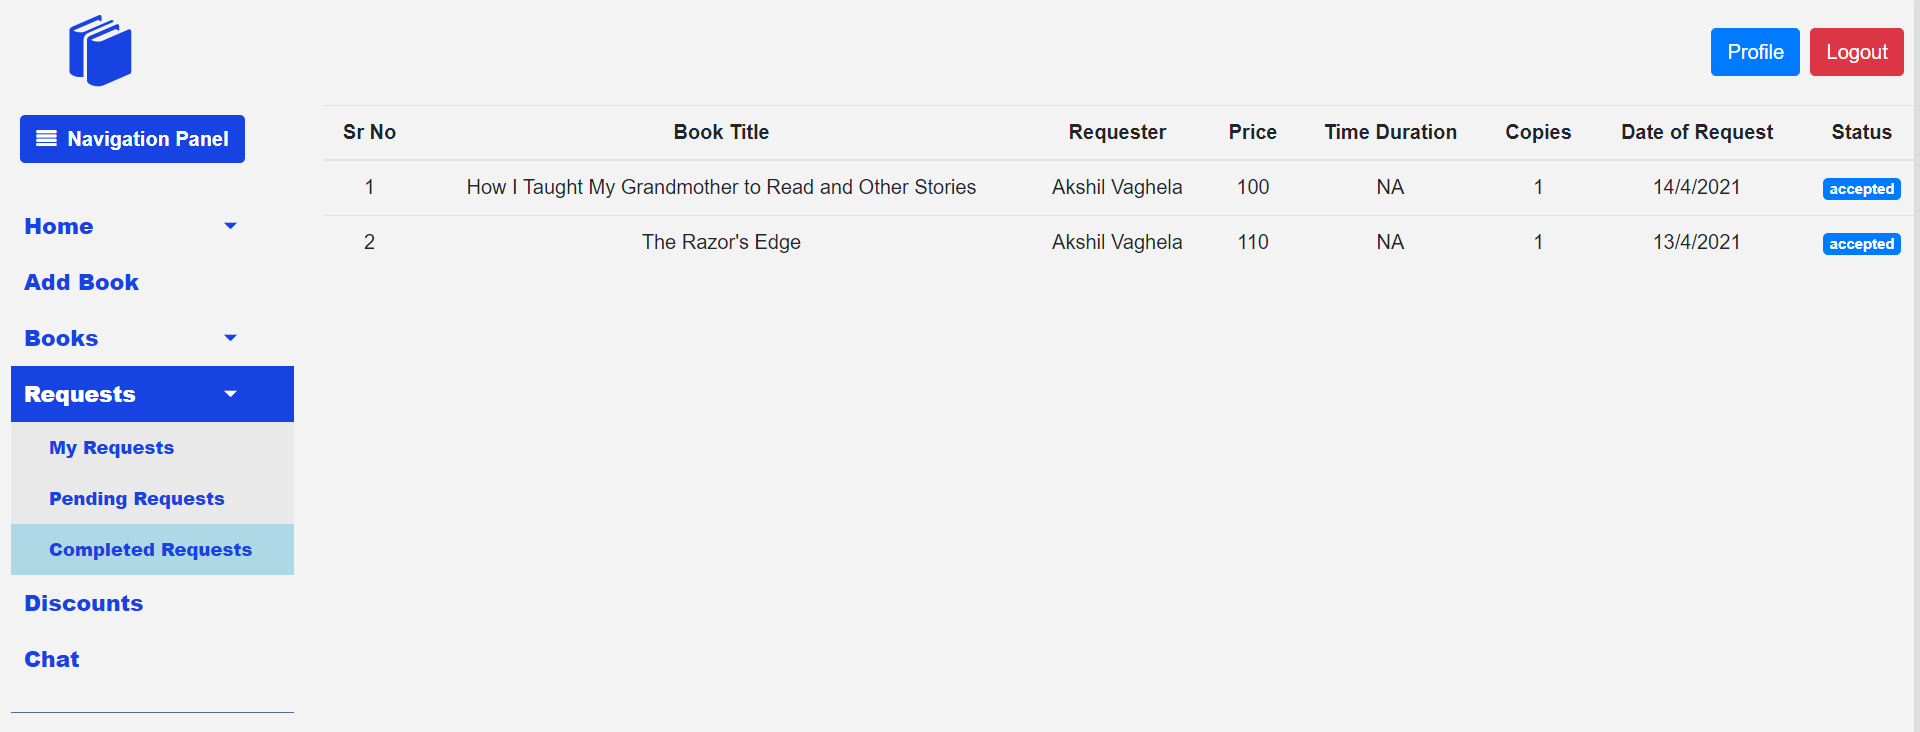
\includegraphics[scale=0.20,margin=2,frame]{completedrequests.PNG}
     \caption{Completed Requests}
     \label{fig:completedrequests}
 \end{figure}

All the above three sections are available for the user part while the \emph{My requests} section won't be available for the vendor.

\subsection{Viewing books involved in transactions}
These books are divided into four categories.

\subsubsection{Books lent}
This section shows the collection of books that you have lent to other users. Clicking on a book here will redirect to a page where the book details as well as details of the users who have borrowed this particular book will be found.
\begin{figure}[h]
     \centering
     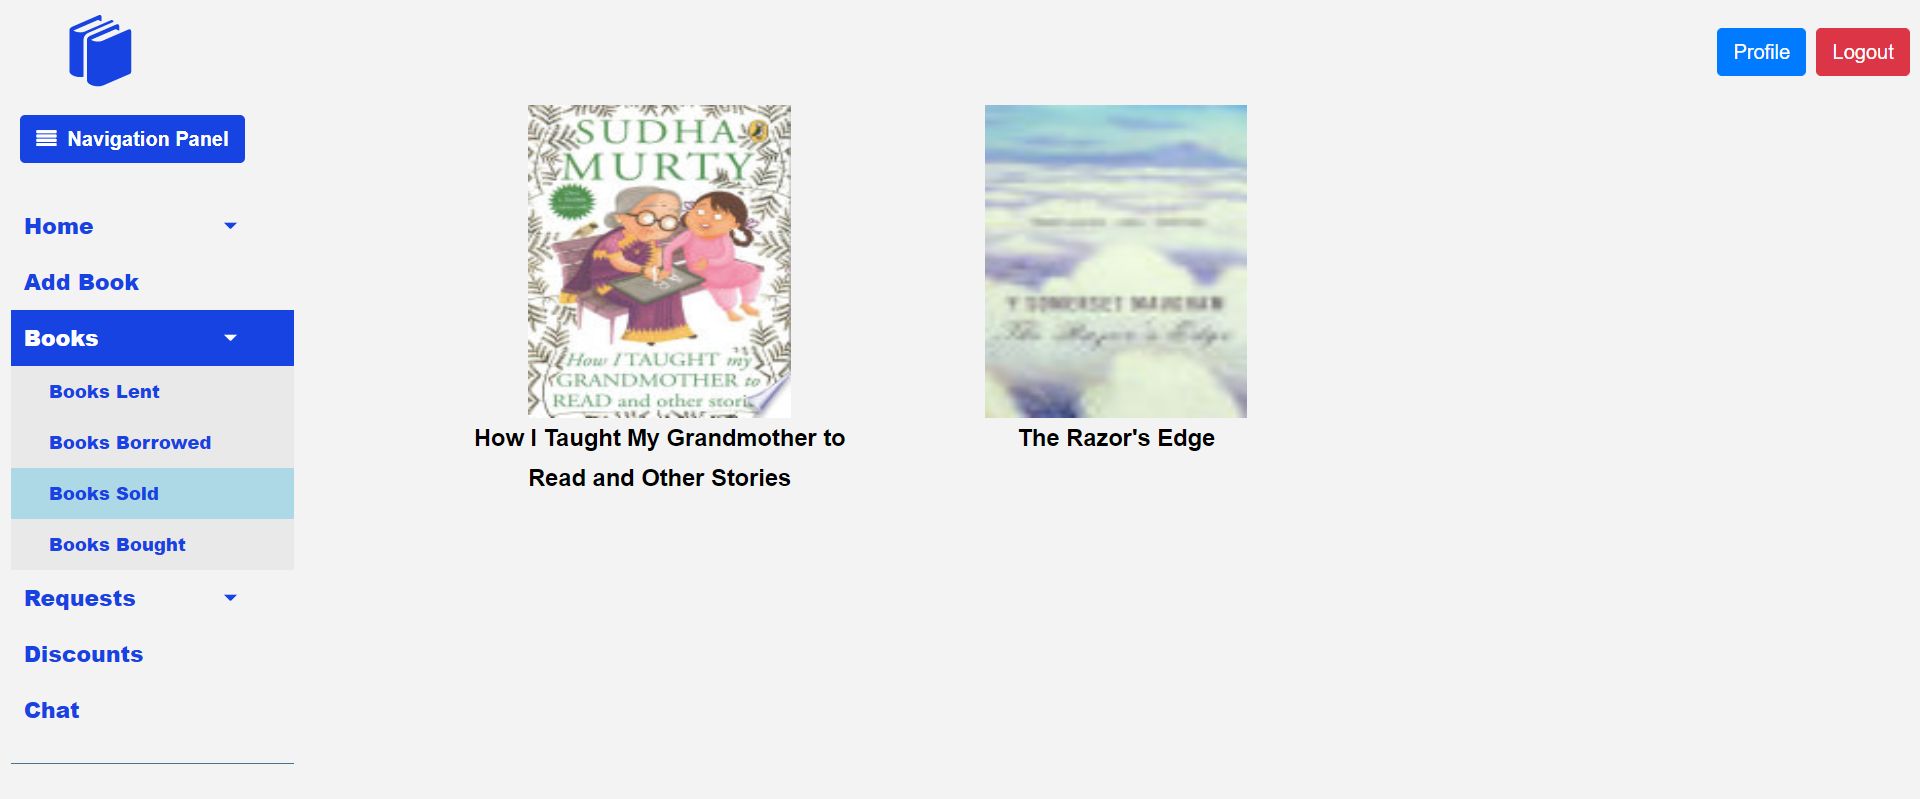
\includegraphics[scale=0.20,margin=2,frame]{Books Sold.PNG}
     \caption{Books Sold}
     \label{fig:booksold}
 \end{figure}
 \begin{figure}[h]
     \centering
     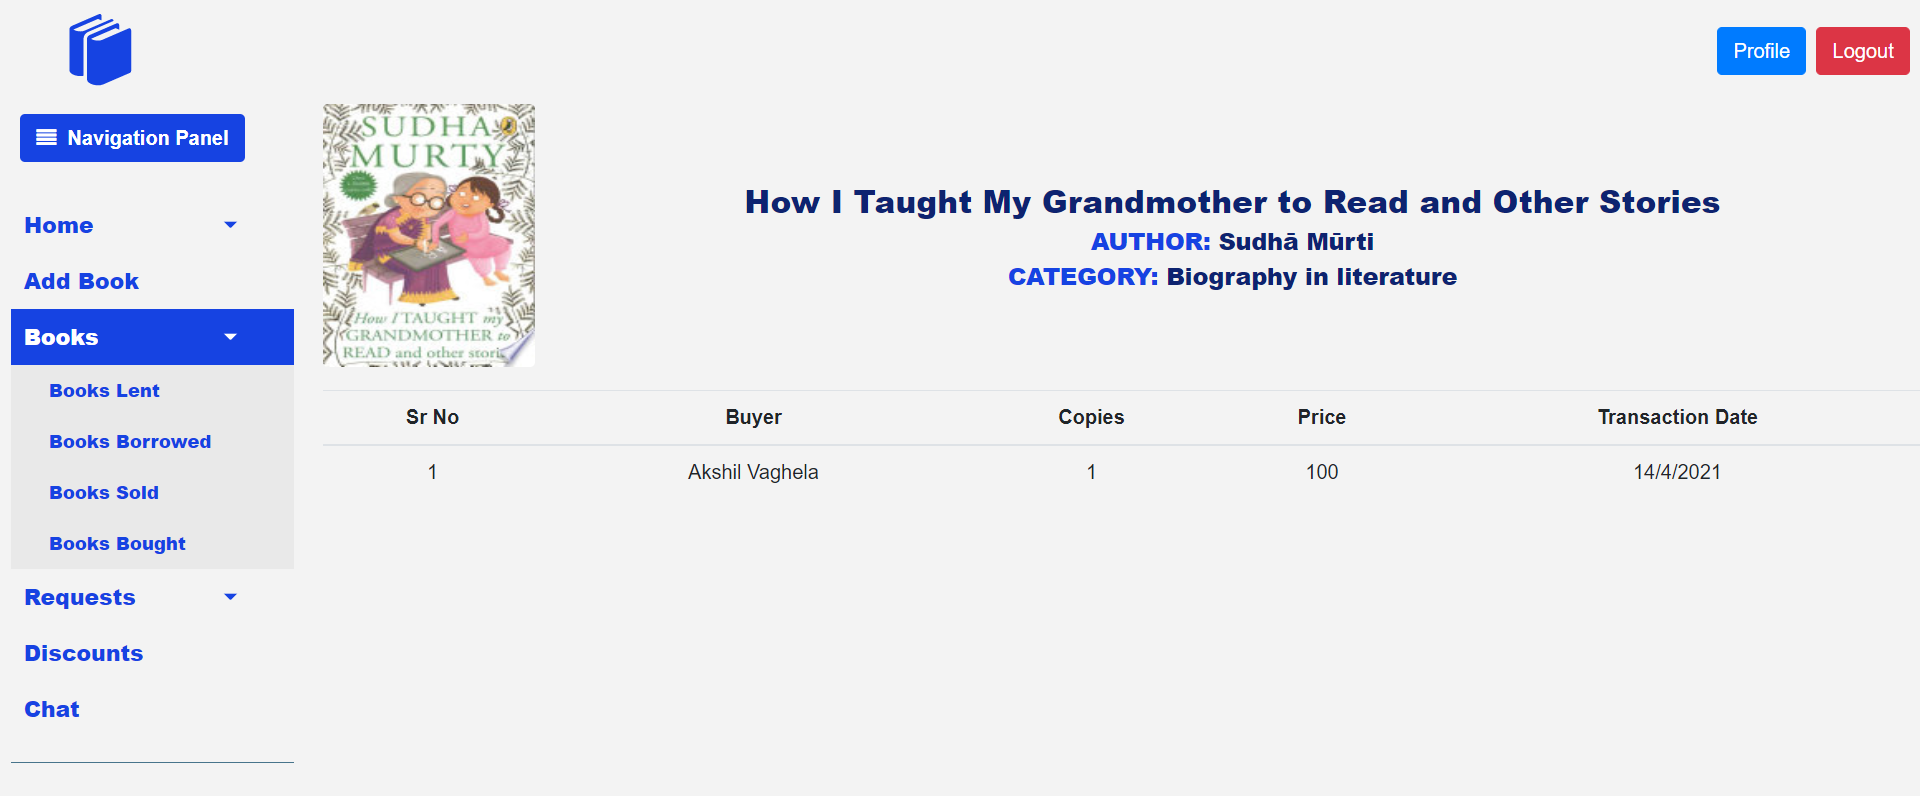
\includegraphics[scale=0.20,margin=2,frame]{individualbooksold.PNG}
     \caption{Books Sold - Individual book page}
     \label{fig:individualbooksold}
 \end{figure}
\subsubsection{Books borrowed}
This section shows the collection of books that the user has borrowed from other users as well as vendors. Each individual book page will show the details of the book and information about the users and vendors who have lent the book.
\subsubsection{Books sold}
This section shows the collection of books that the user has sold to other users. The details of the book as well as details of the buyer, transaction date, price etc will also be shown when a book is clicked as shown in figure \ref{fig:individualbooksold}.
\subsubsection{Books bought}
This section shows the collection of books that the user has bought from other user and vendors. Each individual book page contains information about the seller, date of purchase, price etc along with the book details.

All of these sections are available for the user while only \emph{Books sold} and \emph{Books lent} are shown to the vendor.

\subsection{Return book}
This functionality is a two step return process for returning a borrowed or rented book. When a user visits the profile page of any borrowed/rented book, he/she will get an option to initiate a request to return the book (shown in figure \ref{fig:initiatereturnrequest}).
\begin{figure}[h]
     \centering
     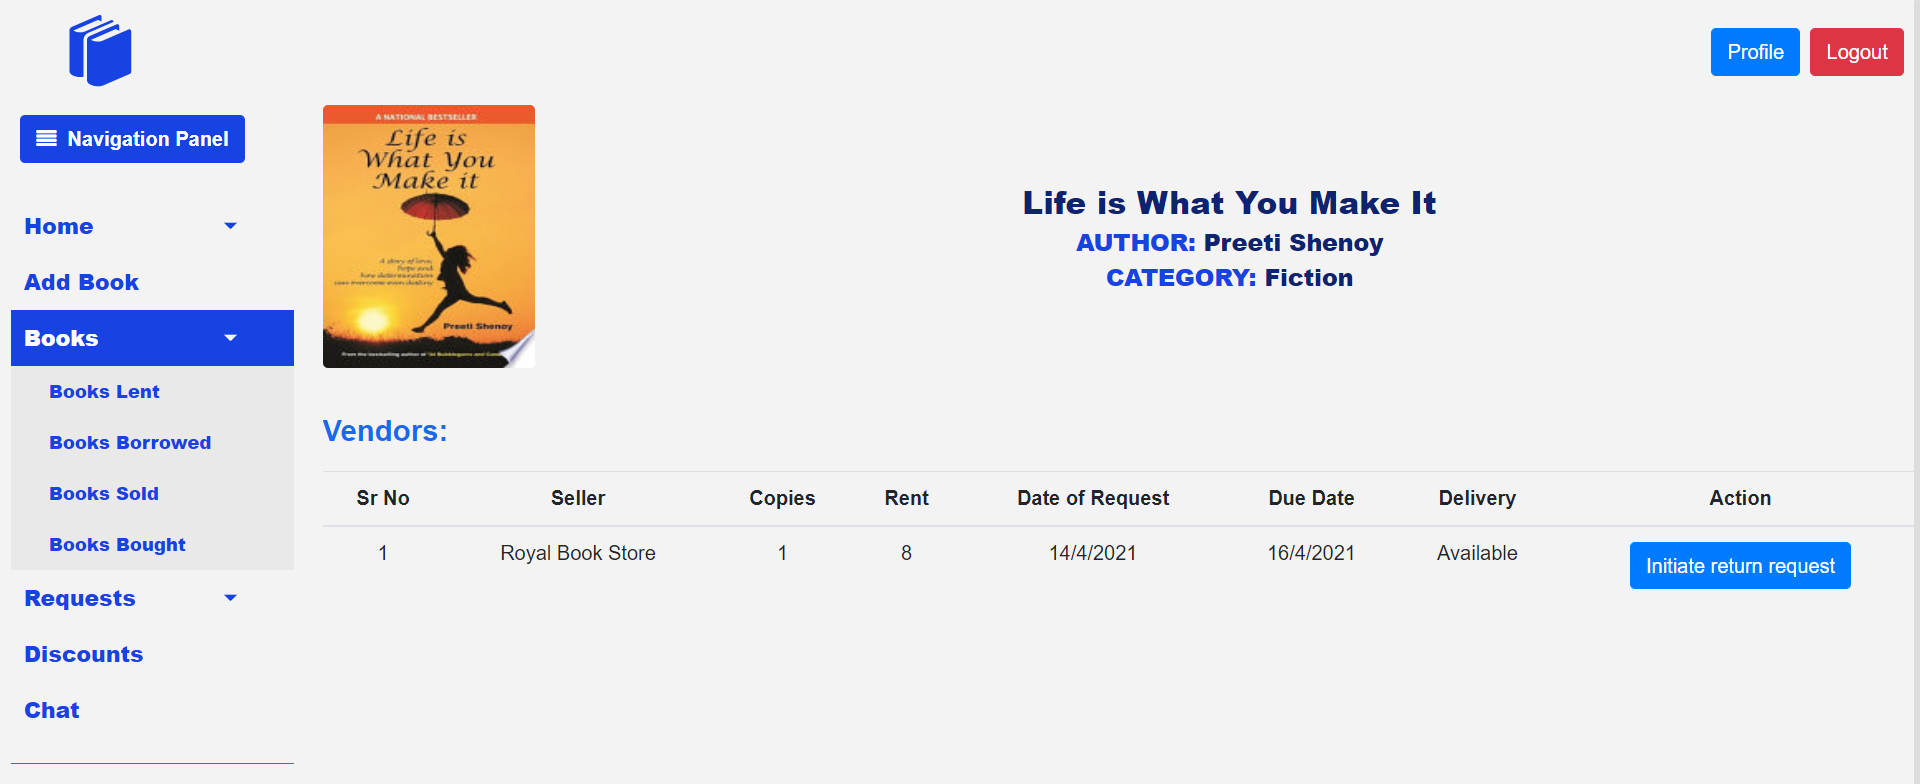
\includegraphics[scale=0.20,margin=2,frame]{initiatereturnrequest.PNG}
     \caption{Initiate return request}
     \label{fig:initiatereturnrequest}
 \end{figure}
As soon as the user clicks that option, the user or vendor who had lend this book will get an option to accept this return request as shown in figure \ref{fig:acceptbookreturn}. 
\begin{figure}[h]
     \centering
     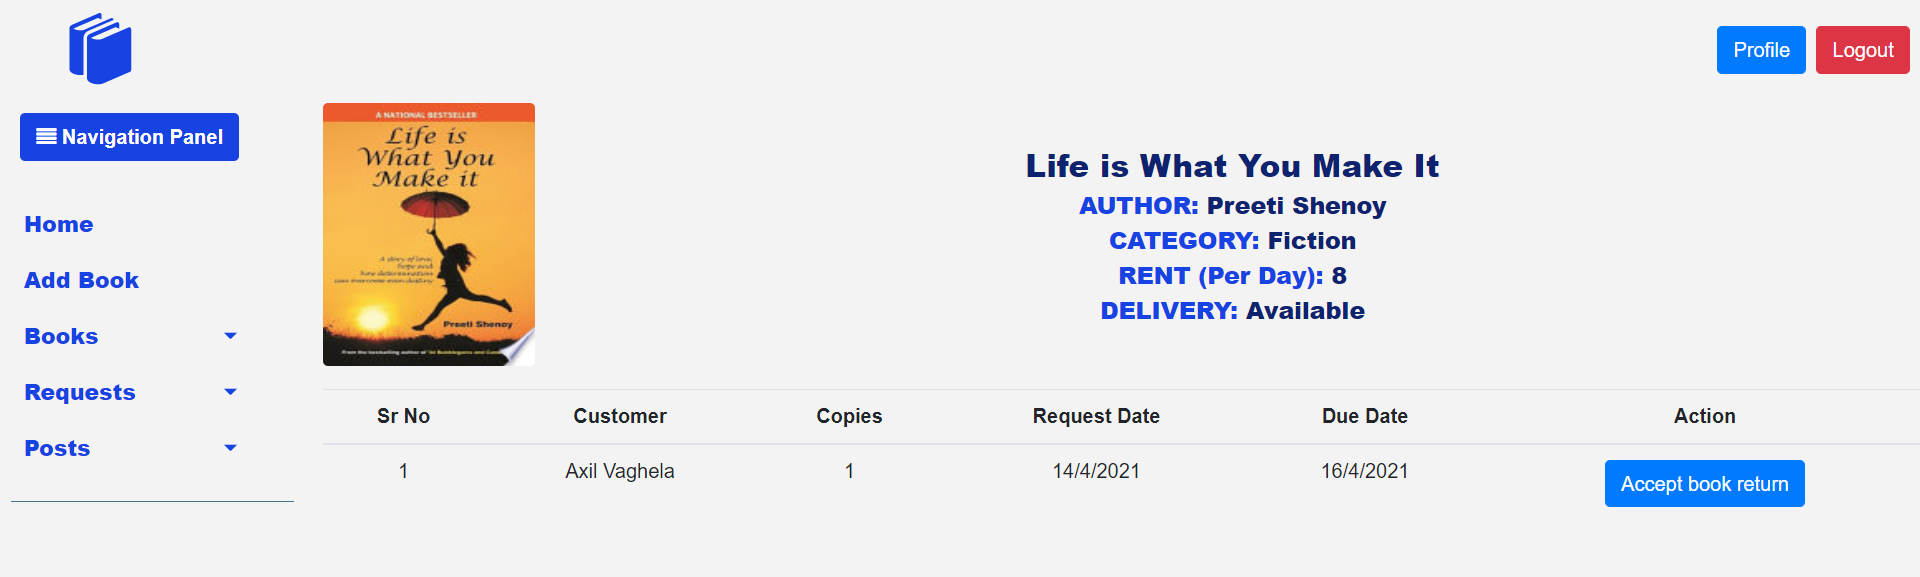
\includegraphics[scale=0.20,margin=2,frame]{acceptbookreturn.PNG}
     \caption{Accept book return}
     \label{fig:acceptbookreturn}
 \end{figure}
When the user/vendor receives his/her copy back he/she can click on this button and the transaction will be marked as complete and the book will be removed from the \emph{Books Borrowed} collection of the borrower and \emph{Books Lent} collection of the lender.

\subsection{Chat}
The chat feature is available for users through which they can talk to other users. This feature will help them contact other users in case of any query regarding their books, transaction, etc. Figure \ref{fig:chat} shows a conversation between two users.
\begin{figure}[h]
     \centering
     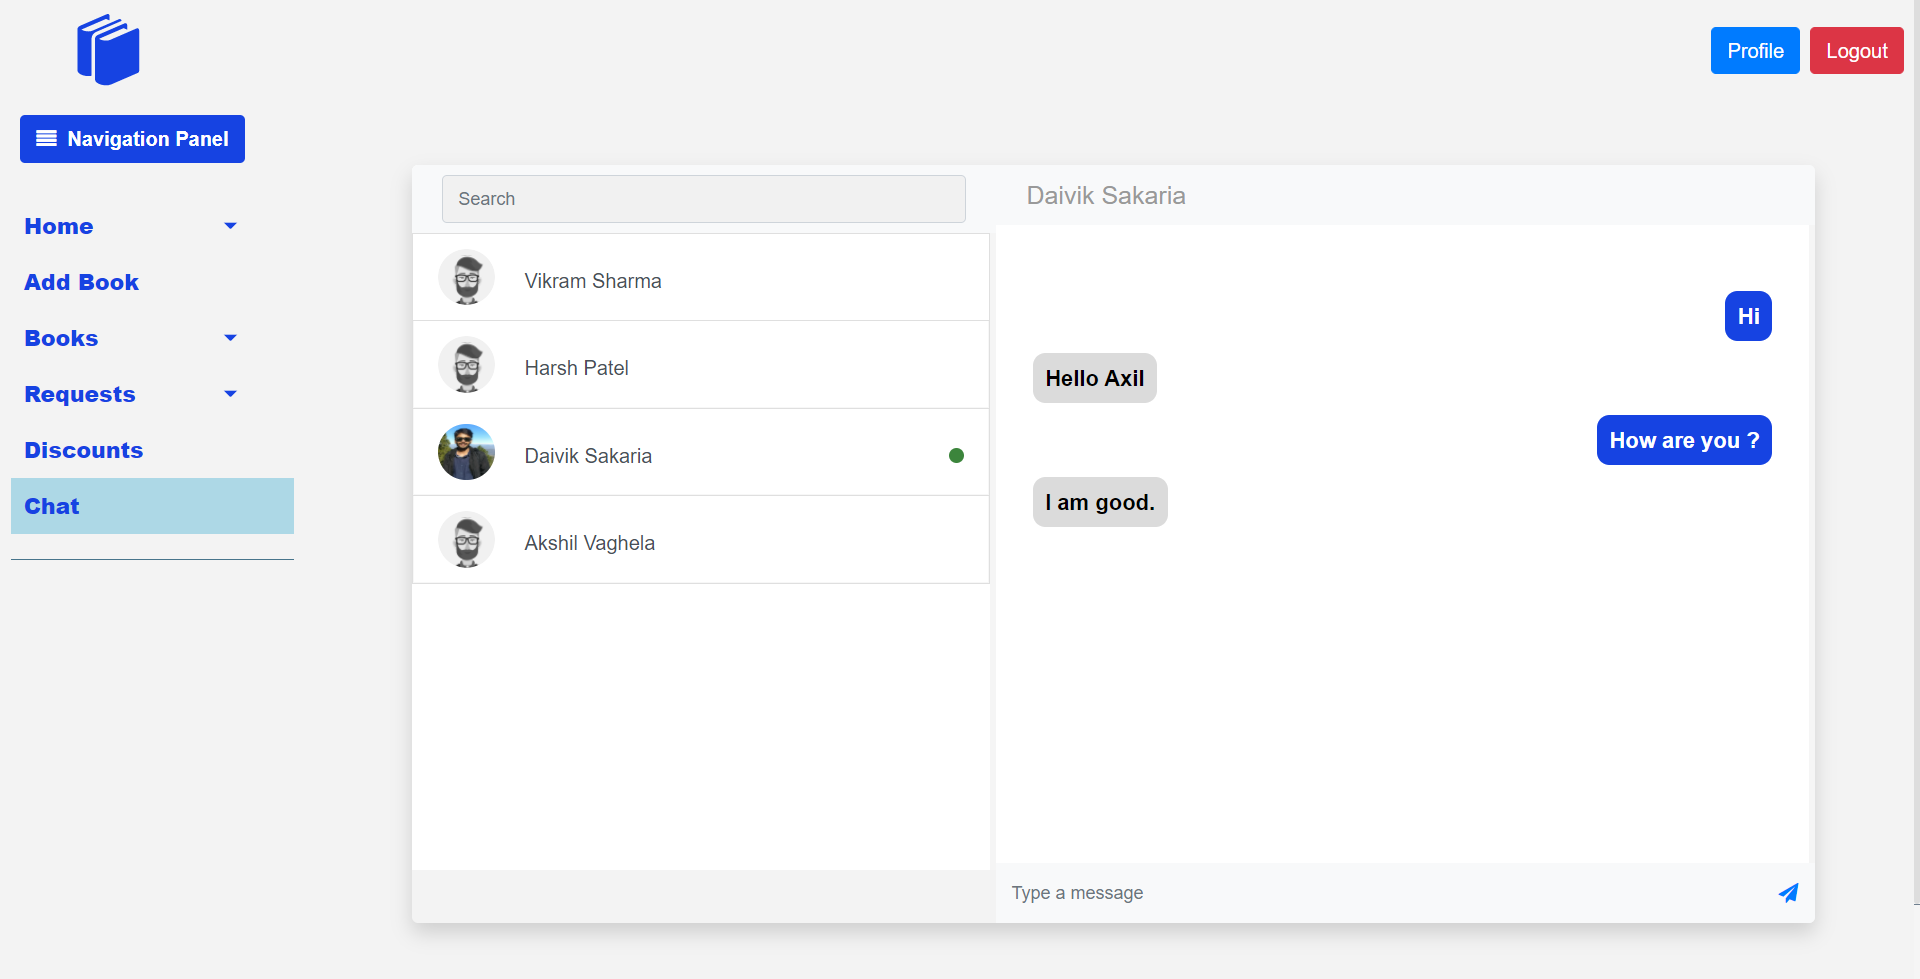
\includegraphics[scale=0.20,margin=2,frame]{chat.PNG}
     \caption{Chat}
     \label{fig:chat}
 \end{figure}

\subsection{Add post}
The \emph{Add post} feature is available for the vendors through which they can notify the users about any discount offers or book sale. 
\begin{figure}[h]
     \centering
     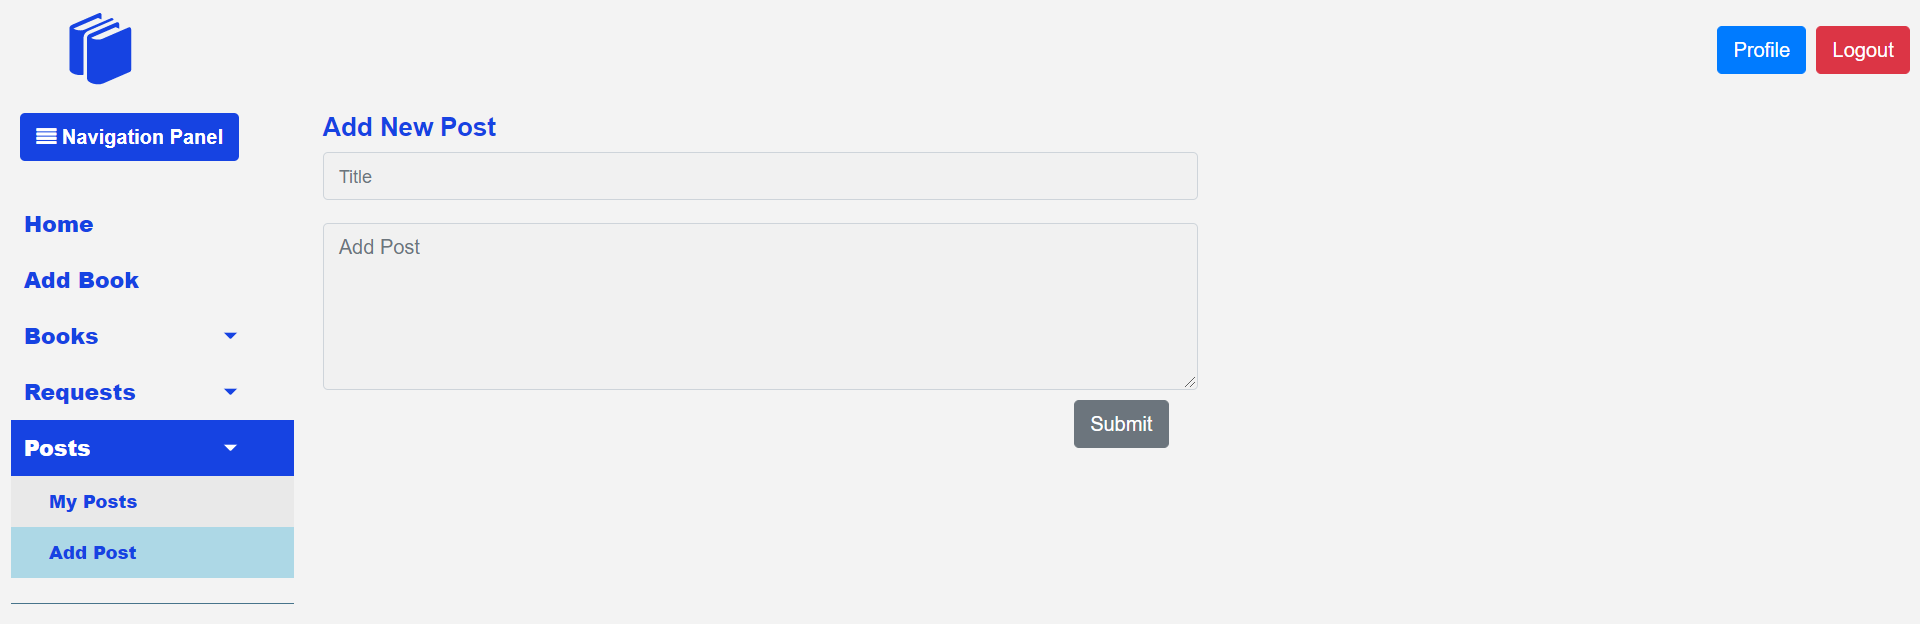
\includegraphics[scale=0.20,margin=2,frame]{addpost.PNG}
     \caption{Add Post}
     \label{fig:addpost}
 \end{figure}
The \emph{Add post} button will redirect the vendor to a new page where the vendor will have to add the title of the post and content of the post. After successful submission, the post will be available to all the users and for the vendor, their posts can be viewed under \emph{My posts} section. 

\subsection{Discounts}
All the posts added by the vendors can be viewed by the users in the \emph{Discounts} section. Each post will contain the fields like shop name, name of the shop owner, post title, etc.
\begin{figure}[h]
     \centering
     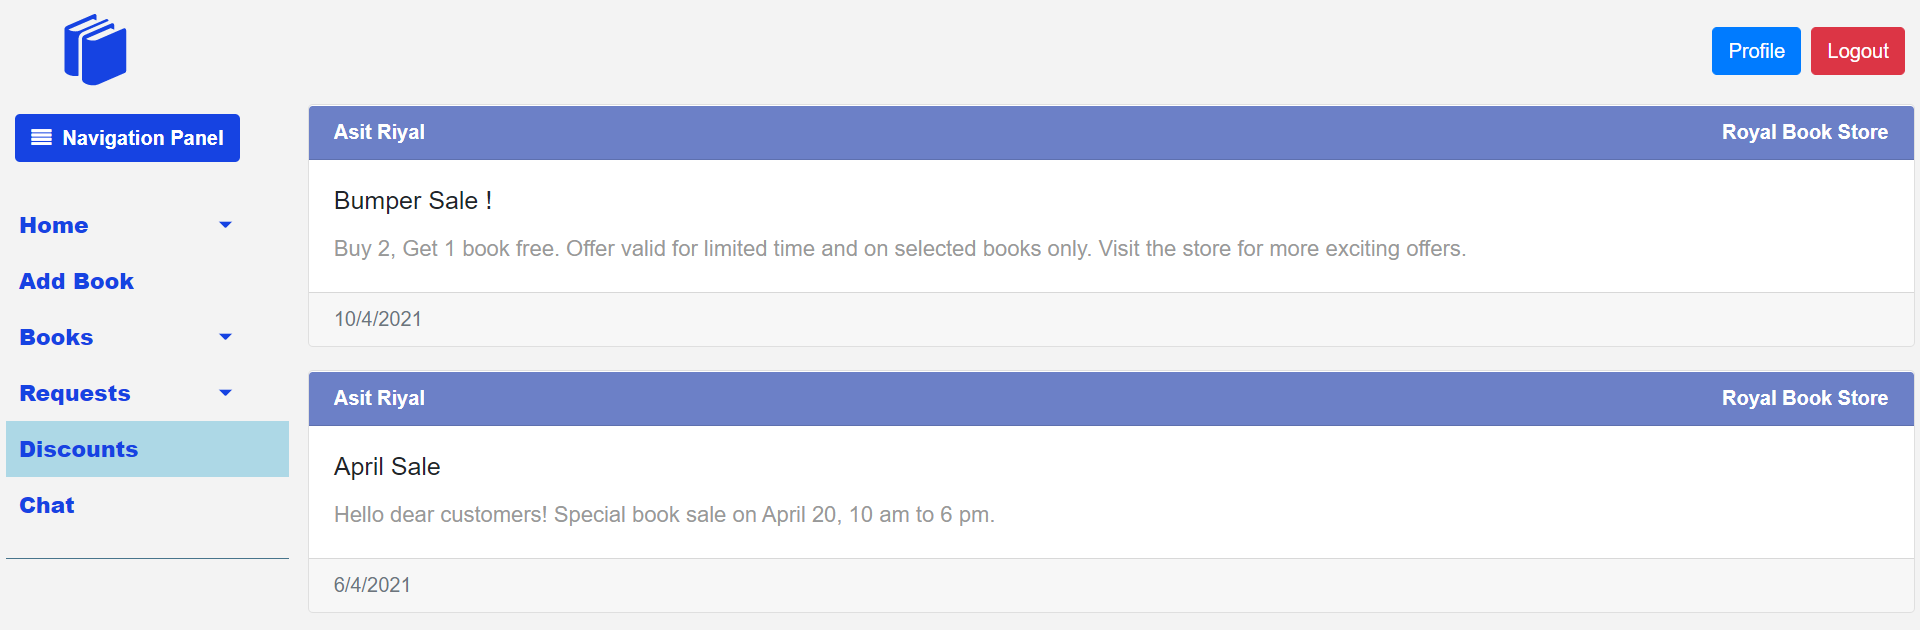
\includegraphics[scale=0.20,margin=2,frame]{discounts.PNG}
     \caption{Discounts}
     \label{fig:discounts}
 \end{figure}

\subsection{Profile}
The \emph{profile} button will redirect the user/vendor to a new page where the user will see their personal details like name, email id, college, bio etc while the vendor will see details like shop name, owner's name, address etc. The user will have the option of editing his/her bio by clicking on the \emph{Edit bio} button and the vendor will have an option of changing the address by clicking on the \emph{Edit address} button.
\begin{figure}[h]
     \centering
     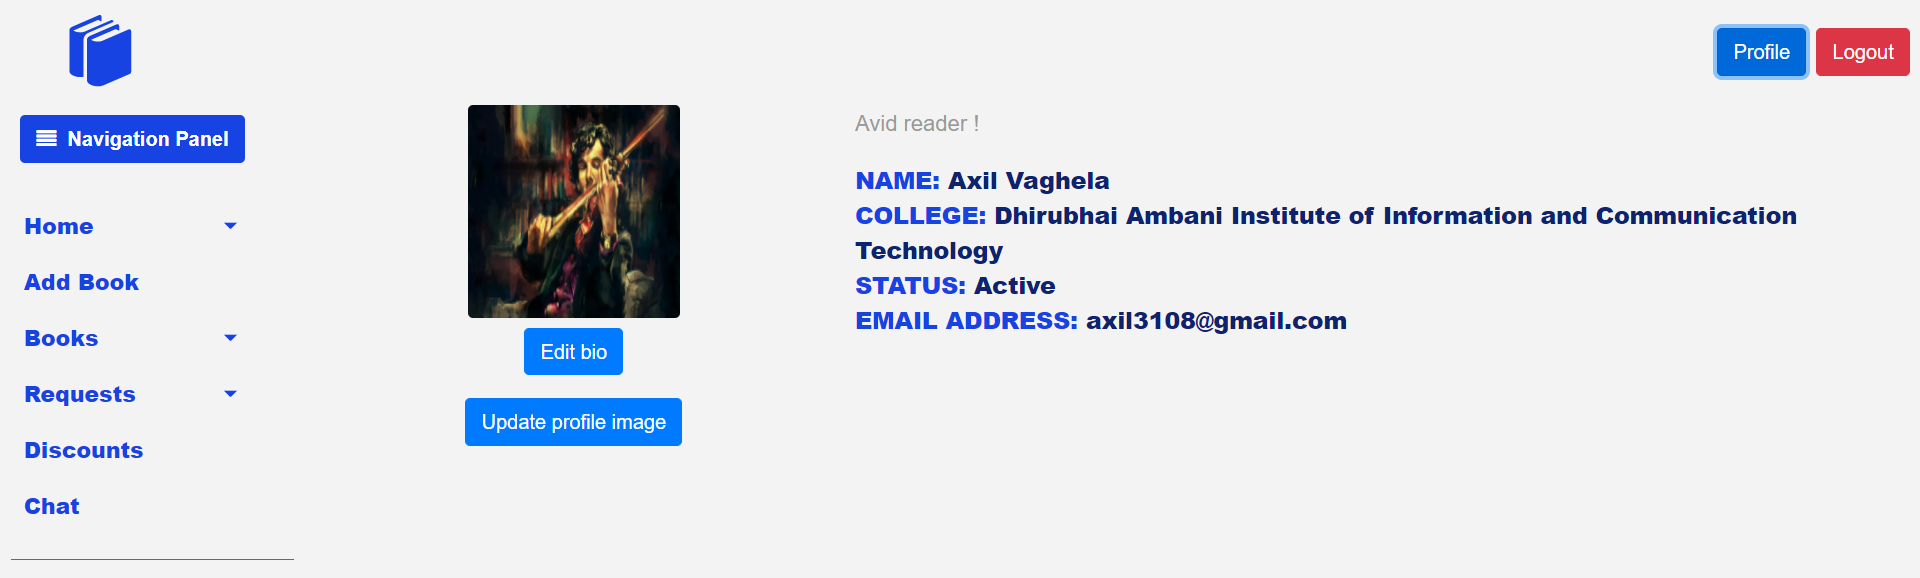
\includegraphics[scale=0.20,margin=2,frame]{profile.PNG}
     \caption{Profile}
     \label{fig:profile}
 \end{figure}

\subsection{Add profile picture}
This functionality helps a user/vendor to upload their profile picture to the system. In their profile page, the user/vendor will get an option of uploading a picture through which they can set their profile picture. If a user/vendor doesn't set their profile picture then a default picture will be shown.
\begin{figure}[h]
     \centering
     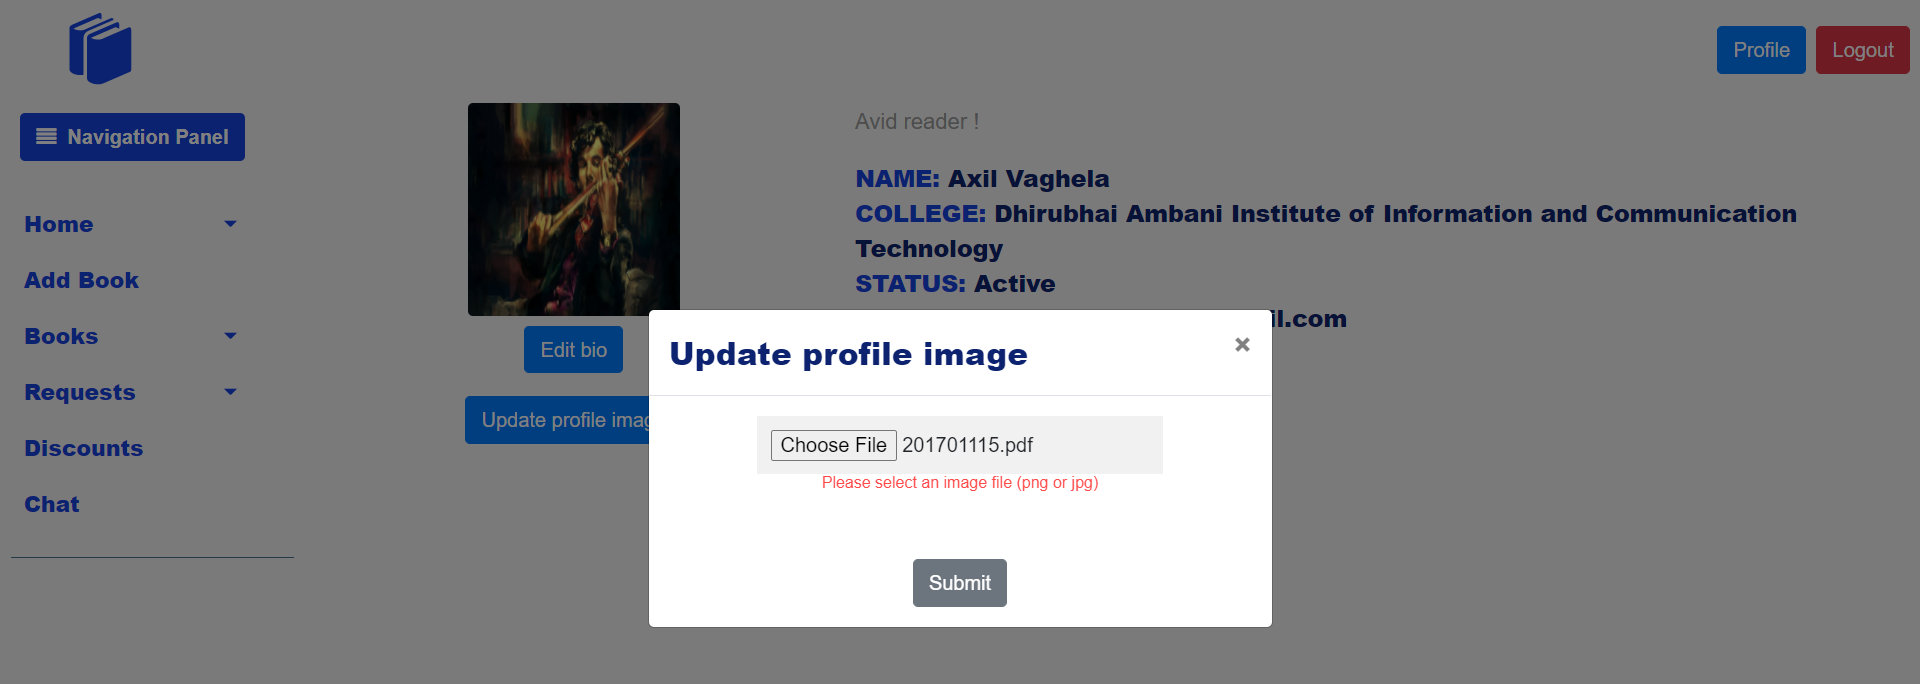
\includegraphics[scale=0.20,margin=2,frame]{profileimage.PNG}
     \caption{Update profile image}
     \label{fig:profilepicture}
 \end{figure}

\subsection{Manage books}
This functionality is available to the Admin. Under the \emph{books} section all the books added to the system(by both users and vendors) will be shown. 
\begin{figure}[h]
     \centering
     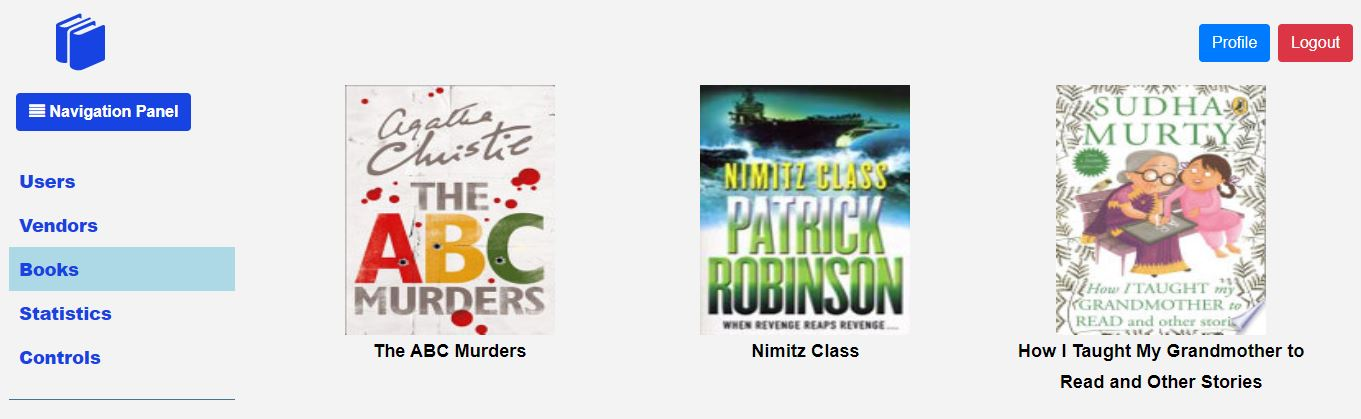
\includegraphics[scale=0.20,,margin=2,frame]{books.JPG}
     \caption{All Books}
     \label{fig:books}
 \end{figure}
Clicking an individual book will redirect the Admin to the details of that book. The book details shown are title, author, status of the book, etc. The Admin will also have an option to \emph{disable} a particular book if for some reason the book violates the policy of the platform.
\begin{figure}[h]
     \centering
     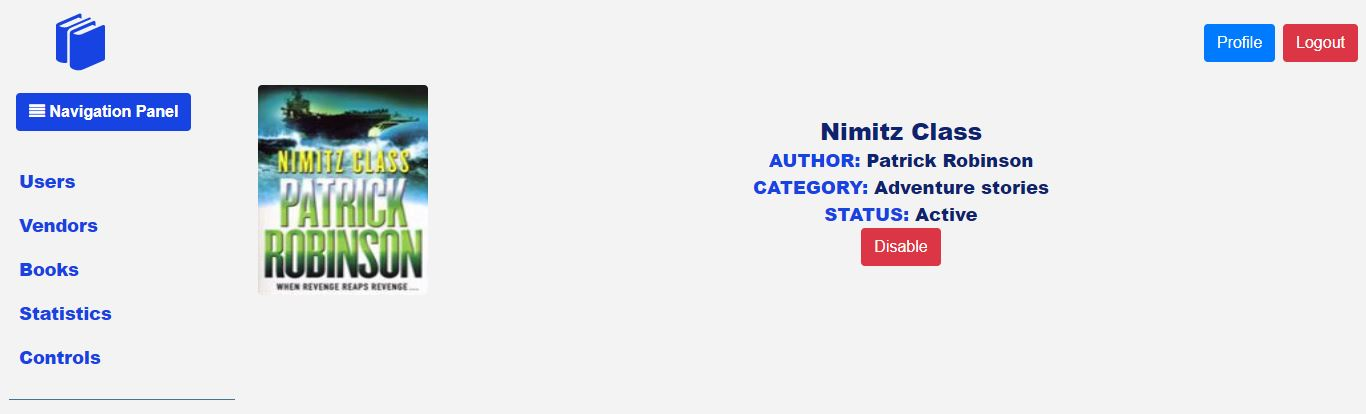
\includegraphics[scale=0.20,margin=2,frame]{individualbookadmin.JPG}
     \caption{Admin - Individual Book}
     \label{fig:individualbook}
 \end{figure}
A disabled book won't be available for any transaction and will be removed from all book collections. The Admin will also have an option to \emph{enable} a disabled book if it no longer violates the policy of the platform.

\subsection{Manage users and vendors}
This functionality is available to the Admin. An Admin can see the list of all users and vendors who have registered on the system.
\begin{figure}[h]
     \centering
     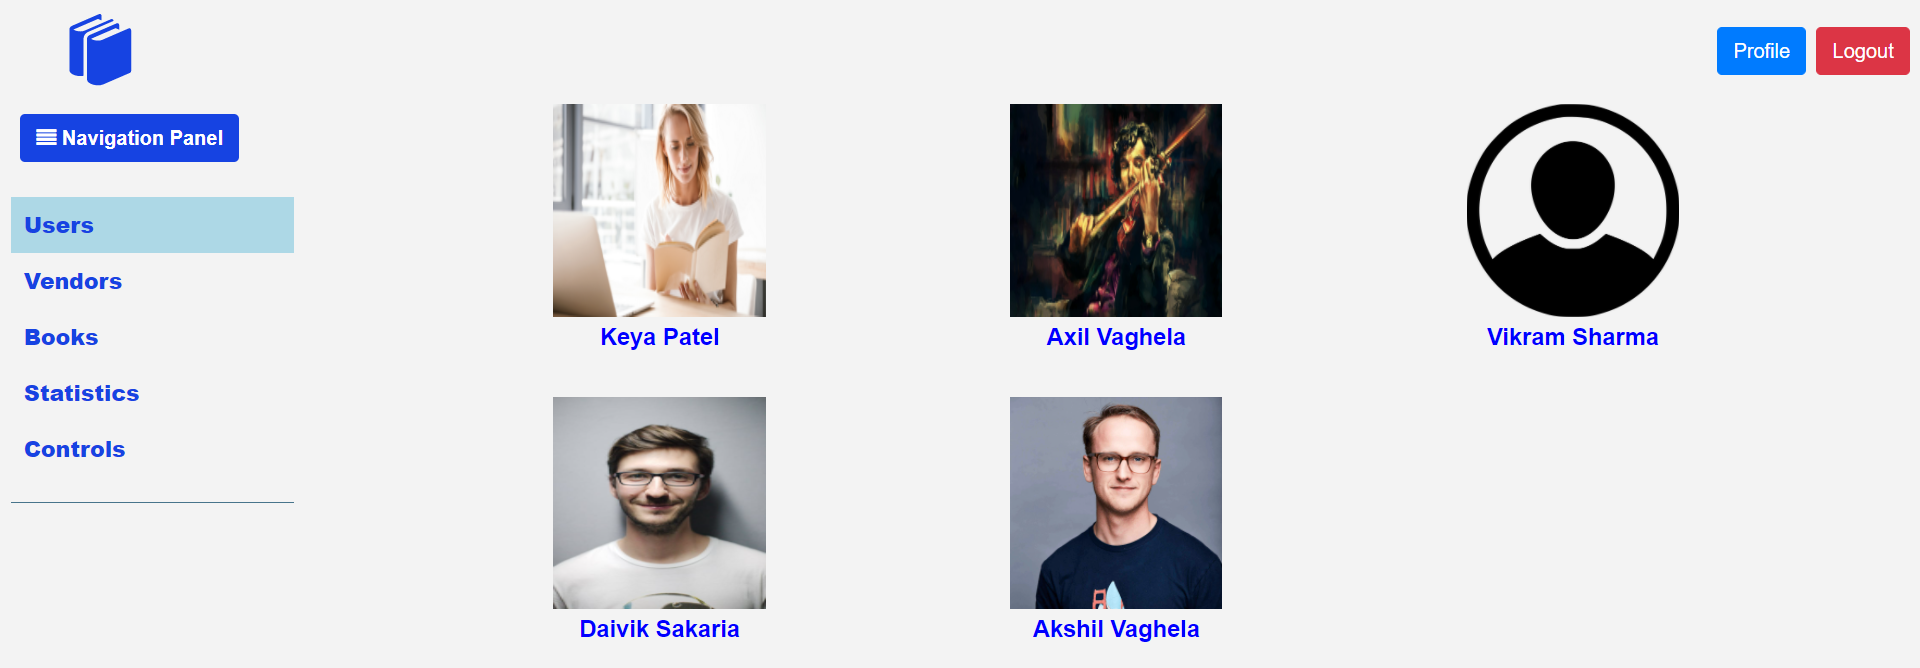
\includegraphics[scale=0.20,margin=2,frame]{users.PNG}
     \caption{Users}
     \label{fig:users}
 \end{figure}
Clicking on a particular user/vendor will take the Admin to their profile page where all their details will be displayed. 
\begin{figure}[h]
     \centering
     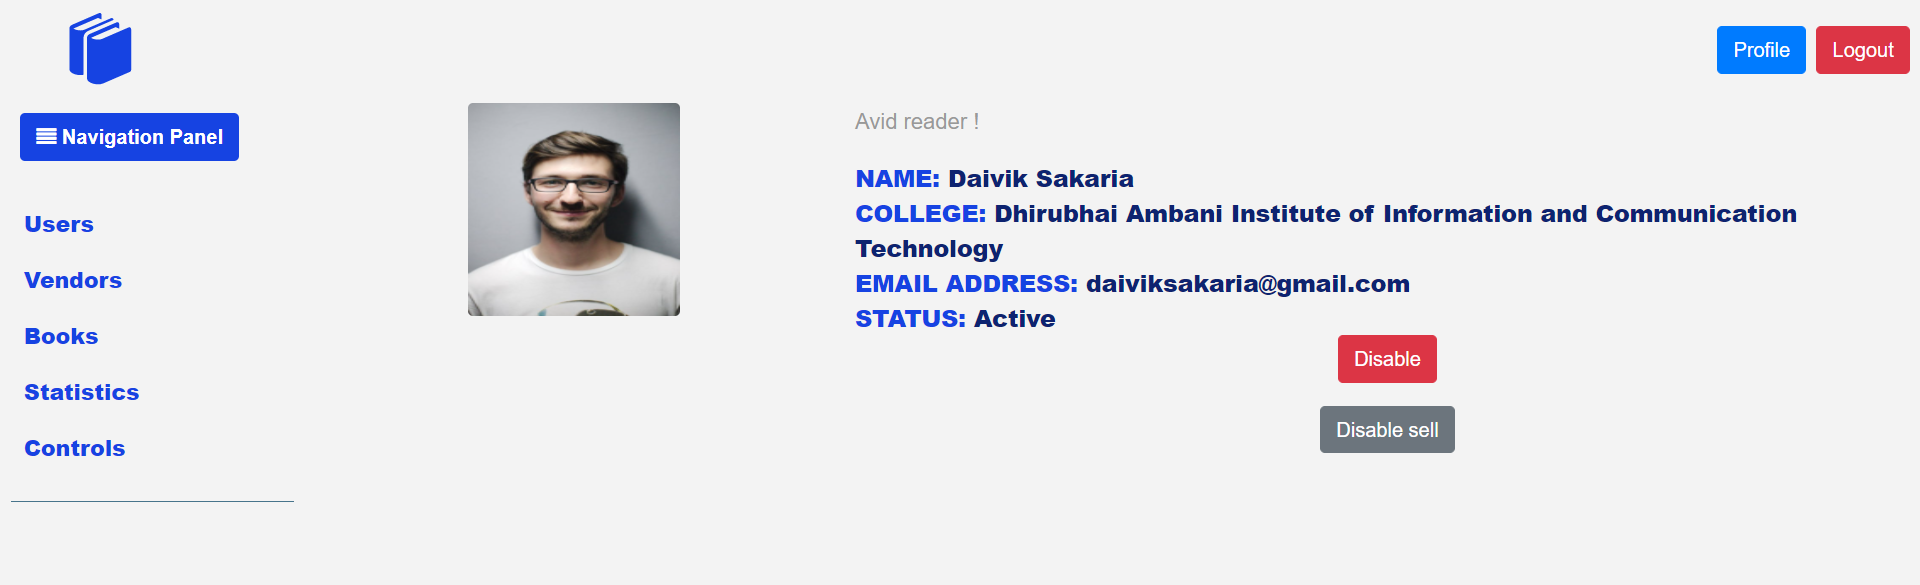
\includegraphics[scale=0.20,margin=2,frame]{Userprofile.PNG}
     \caption{User Profile}
     \label{fig:userprofile}
 \end{figure}
The Admin will have an option of deactivating a user/vendor's account if they violate any of the platform guidelines. When a user/vendor's account will be deactivated they won't be able to log in into the system and involve in any transaction. The Admin will also have an option to re-activate a user/vendor's account. The Admin can also enable/disable the Sell feature that allows a user to sell their books on the platform.

\subsection{View statistics}
This functionality enables the Admin to get some insight about the statistics and usage of the platform. \emph{Statistics} will show some of the information like total number of users/vendors, number of active users/vendors, trending books etc.
\begin{figure}[h]
     \centering
     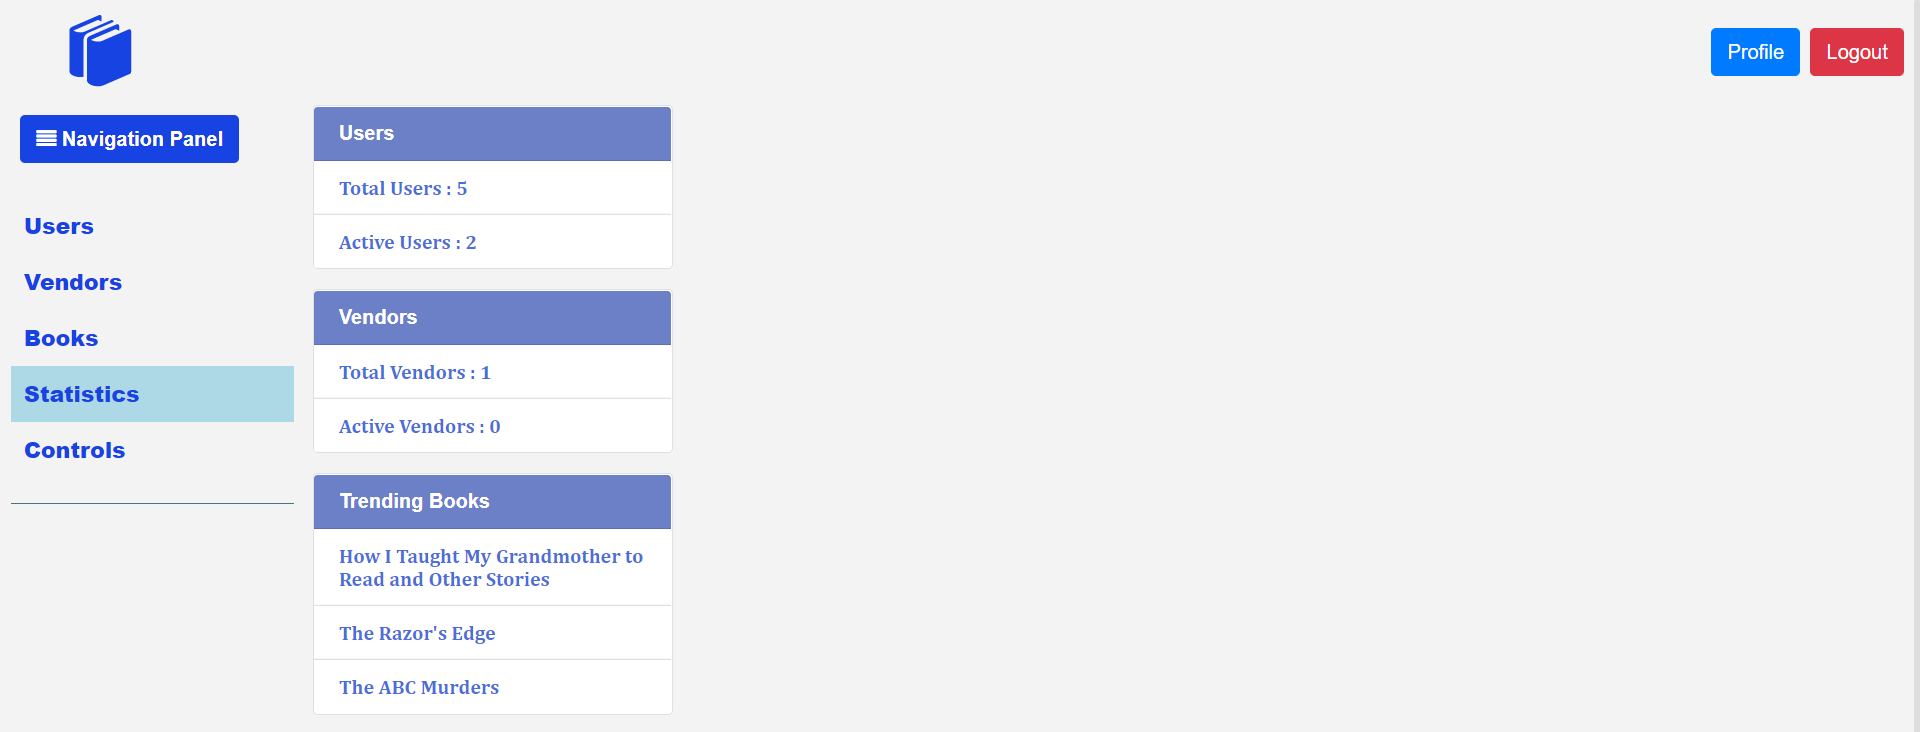
\includegraphics[scale=0.20,margin=2,frame]{statistics.PNG}
     \caption{Statistics}
     \label{fig:statistics}
 \end{figure}

\subsection{Controls}
The Admin has the control over the sell feature offered by the system. For any user, the admin has the authority to turn off/on the sell feature for a particular user. Also the admin has the authority to enable/disable the sell feature for all the DAIICT students as shown in the below figure.  
\begin{figure}[h]
     \centering
     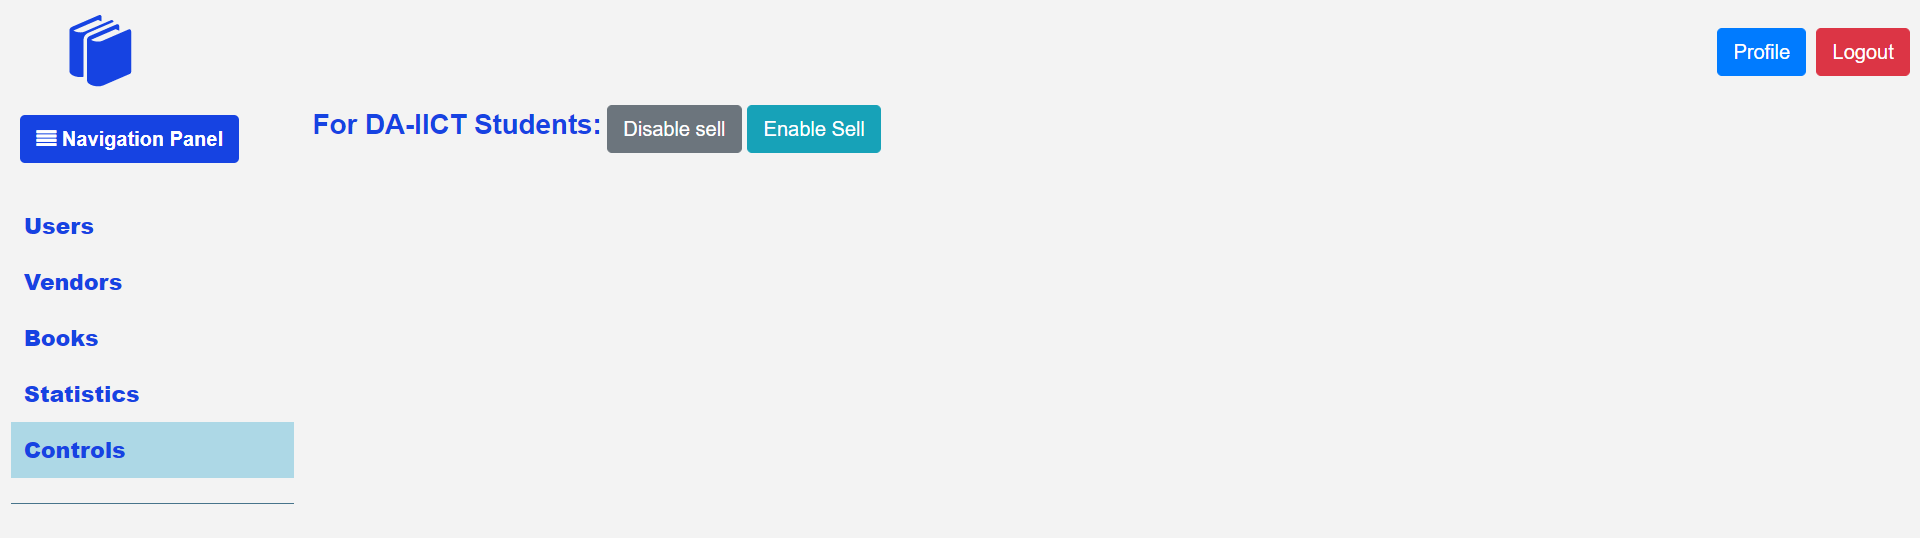
\includegraphics[scale=0.20,,margin=2,frame]{controls.PNG}
     \caption{Controls}
     \label{fig:controls}
 \end{figure}

\section{Implementation}
After finalizing all the functionalities and preparing the required UML diagrams we moved on to the development phase. We have used MVC (Model-View-Controller) architectural model where Model stands for different entity classes, View stands for the web pages i.e what we see and Controller is the component that binds everything together  and runs the application. Here React forms the View part of the MVC. The architecture diagram of our application is shown in figure \ref{fig:architecturediagram}.
\begin{figure}[H]
     \centering
     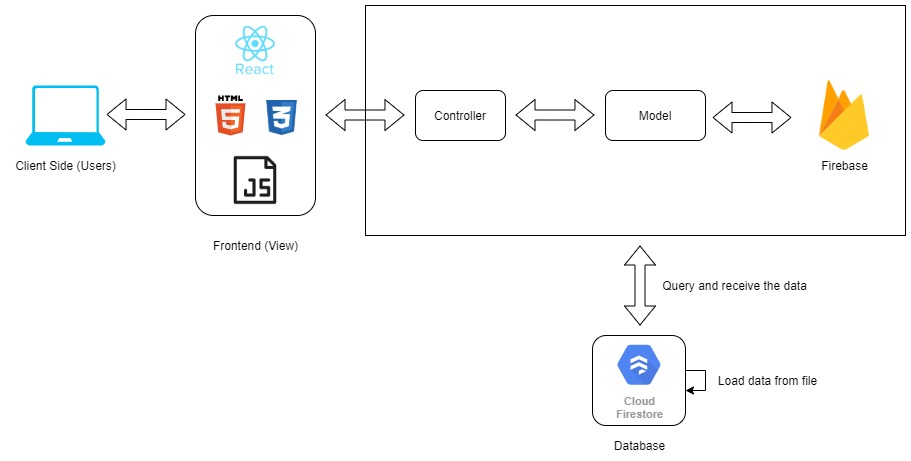
\includegraphics[scale=0.25,,margin=2,frame]{Architecture Diagram.jpg}
     \caption{Architecture Diagram}
     \label{fig:architecturediagram}
 \end{figure}
The comprehensive implementation details is given below.
\subsection{Frontend}
With all the requirements at hand, we looked for various technologies, frameworks that would suit our project. The front-end of the Web Application is developed using HTML, CSS, Javascript and React which is a Javascript library for building interfaces. We have also used Bootstrap to make the Web Application responsive and easy to use on all devices. Some components have also been imported from Material-UI which is a popular React UI framework.
\subsection{Backend}
The back-end of the system is done using Google Firebase. Firebase also provides the authentication service through which all the users are authenticated and verified. 
\subsection{Database design}
We had explored various options initially for the database of the system like MongoDB, PostgreSQL, etc. Finally we settled with cloud firestore which is a scalable NoSQL cloud Database provided by Firebase and Google Cloud.

Cloud Firestore is NoSQL database so the data is stored in documents which are organized in collections. It is a schemaless database so each document belonging to the same collection can also have different fields. Our database consists of nine top level collections where each collection contains several documents. Figure \ref{fig:databasedesign} shows the structure and design of our database.
\begin{figure}[h]
     \centering
     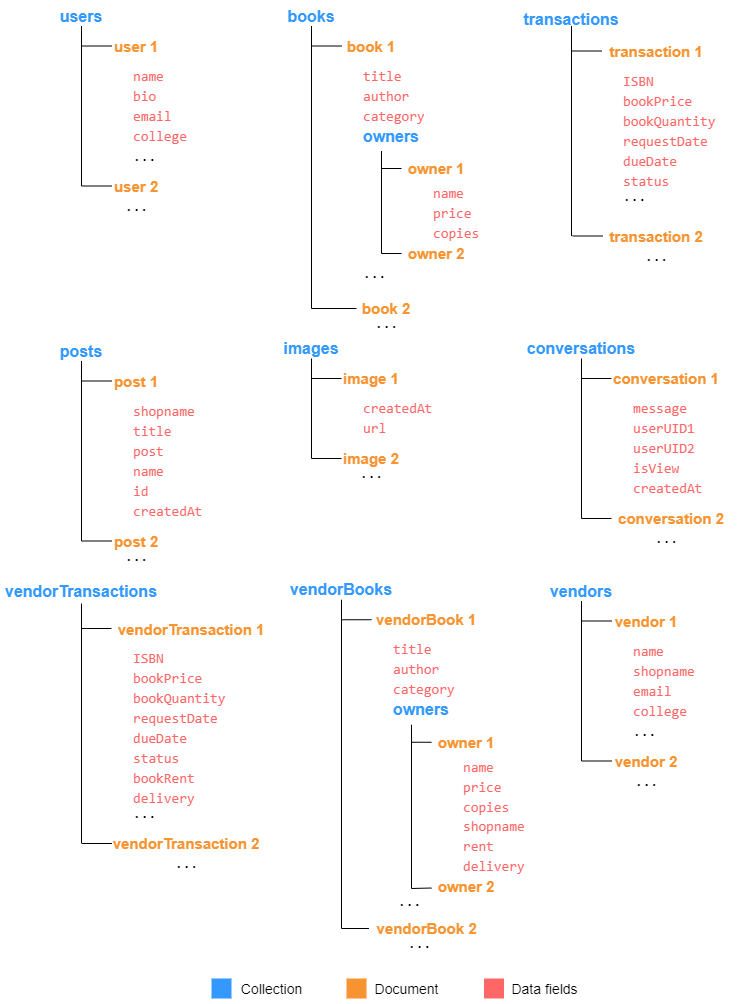
\includegraphics[scale=0.30,margin=2,frame]{Database-design.png}
     \caption{Database Design}
     \label{fig:databasedesign}
 \end{figure}
 
\section{Testing}
Testing is a crucial part of the development process followed during the development of a Web Application. Initially during the development phase, we followed the basics of functional testing and tested each feature individually. The motive behind functional testing was to make sure the features or functionalities that we are developing are flawless and reliable. Eventually we would be integrating all of the features together, so the focus was to test all the features individually first so that the chances of bugs would be reduced after integrating the all the features. So we tested each feature against all the possible test cases as soon we developed it and made sure they run smoothly. After developing the entire system, the focus was then on testing the system as whole and for that we used black box testing where we shifted our focus on testing the whole system. During the initial phase we made several user and vendor accounts ourselves and tried testing various functionalities of the system by exposing the system to various scenarios. We did find some bugs and irregularities during the initial phase and made some improvements to make the system more efficient and robust. Afterwards, we took feedback from various other users and improved the system accordingly. We followed a similar process quite a few times and tried to make the system as smooth and efficient as possible. The test results of the screen shown in figure \ref{fig:requestbookfeature} is presented in table \ref{table:1}. All the other screens have also been tested similarly.

\begin{figure}[H]
     \centering
     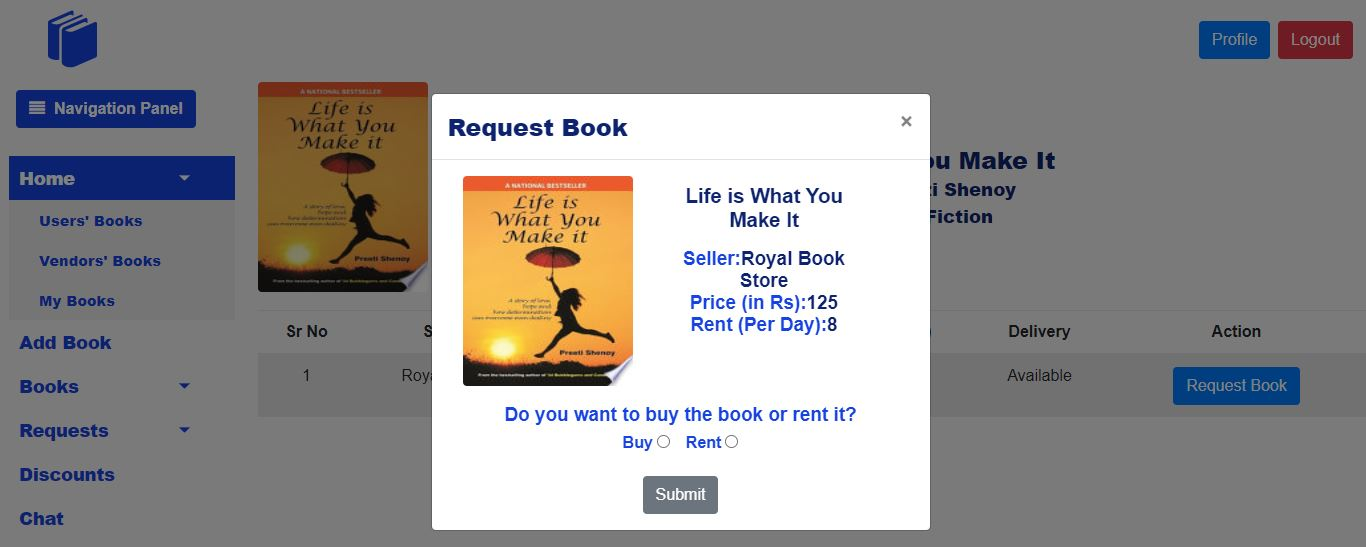
\includegraphics[scale=0.23,margin=2,frame]{testing.JPG}
     \caption{Request Book}
     \label{fig:requestbookfeature}
 \end{figure}

\begin{table}[H]
\centering
\begin{tabularx}{0.50\textwidth}{|>{\centering\arraybackslash}X | >{\centering\arraybackslash}X  | >{\centering\arraybackslash}X  | >{\centering\arraybackslash}X  | >{\centering\arraybackslash}X  | >{\centering\arraybackslash}X  | >{\centering\arraybackslash}X|} 
 \hline
 Test case & Action & Inputs & Expected output & Actual Output & Test Result \\ [0.5ex] 
 \hline\hline
 1a Request book - buy & Click on the buy option & Enter Quantity: 1 & Book requested & Book requested & Pass \\ 
 \hline
 1b Request book - buy & Click on the buy option & Enter Quantity: 5 & Book limit exceeded & Book limit exceeded & Pass\\
 \hline
 1c Request book - buy & Click on the buy option & Enter Quantity: null & Error - Please enter quantity & Error - Please enter quantity & Pass\\
 \hline
 2a Request Book - rent & Click on the rent option & Quantity: 5, Time duration: 2 days & Book request sent & Book request sent & Pass\\
 \hline
 2b Request Book - rent & Click on the rent option & Quantity: 5, Time duration: null & Error - Enter time duration & Error - Enter time duration & Pass\\
 \hline
 2c Request Book - rent & Click on the rent option & Quantity:10, Time duration: 5 days & Book limit exceeded & Book limit exceeded & Pass\\
 \hline
\end{tabularx}
\newline
\caption{Testing - Request Book}
\label{table:1}
\end{table}

\section{Conclusion and Future Works}
The web application at present can handle lending and borrowing books among each other. Users can also buy or sell books to each other. Vendors can also use this system to rent or sell books to users. 
Having said that, there is scope of improving the login functionality of website, in a sense that a person can toggle between his/her user and vendor profile from a single logged in account itself. Currently, a person has to make 2 different accounts if he/she wants to be an user and vendor both. Also the system currently doesn't support reminder mails due to some implementation limitations. The system also supports some additional features for the DA-IICT students where the Admin can control if a student can sell a book or not. This functionality can be scaled across colleges where each college can have a Admin who would able to monitor as well as control the transactions occurring within their college. This would help the colleges use this platform locally and enhance their user experience. 

% \subsection{Abbreviations and Acronyms}\label{AA}
% Define abbreviations and acronyms the first time they are used in the text,
% even after they have been defined in the abstract. Abbreviations such as
% IEEE, SI, MKS, CGS, ac, dc, and rms do not have to be defined. Do not use
% abbreviations in the title or heads unless they are unavoidable.

% \subsection{Units}
% \begin{itemize}
% \item Use either SI (MKS) or CGS as primary units. (SI units are encouraged.) English units may be used as secondary units (in parentheses). An exception would be the use of English units as identifiers in trade, such as ``3.5-inch disk drive''.
% \item Avoid combining SI and CGS units, such as current in amperes and magnetic field in oersteds. This often leads to confusion because equations do not balance dimensionally. If you must use mixed units, clearly state the units for each quantity that you use in an equation.
% \item Do not mix complete spellings and abbreviations of units: ``Wb/m\textsuperscript{2}'' or ``webers per square meter'', not ``webers/m\textsuperscript{2}''. Spell out units when they appear in text: ``. . . a few henries'', not ``. . . a few H''.
% \item Use a zero before decimal points: ``0.25'', not ``.25''. Use ``cm\textsuperscript{3}'', not ``cc''.)
% \end{itemize}

% \subsection{Equations}
% Number equations consecutively. To make your
% equations more compact, you may use the solidus (~/~), the exp function, or
% appropriate exponents. Italicize Roman symbols for quantities and variables,
% but not Greek symbols. Use a long dash rather than a hyphen for a minus
% sign. Punctuate equations with commas or periods when they are part of a
% sentence, as in:
% \begin{equation}
% a+b=\gamma\label{eq}
% \end{equation}

% Be sure that the
% symbols in your equation have been defined before or immediately following
% the equation. Use ``\eqref{eq}'', not ``Eq.~\eqref{eq}'' or ``equation \eqref{eq}'', except at
% the beginning of a sentence: ``Equation \eqref{eq} is . . .''

% \subsection{\LaTeX-Specific Advice}

% Please use ``soft'' (e.g., \verb|\eqref{Eq}|) cross references instead
% of ``hard'' references (e.g., \verb|(1)|). That will make it possible
% to combine sections, add equations, or change the order of figures or
% citations without having to go through the file line by line.

% Please don't use the \verb|{eqnarray}| equation environment. Use
% \verb|{align}| or \verb|{IEEEeqnarray}| instead. The \verb|{eqnarray}|
% environment leaves unsightly spaces around relation symbols.

% Please note that the \verb|{subequations}| environment in {\LaTeX}
% will increment the main equation counter even when there are no
% equation numbers displayed. If you forget that, you might write an
% article in which the equation numbers skip from (17) to (20), causing
% the copy editors to wonder if you've discovered a new method of
% counting.

% {\BibTeX} does not work by magic. It doesn't get the bibliographic
% data from thin air but from .bib files. If you use {\BibTeX} to produce a
% bibliography you must send the .bib files.

% {\LaTeX} can't read your mind. If you assign the same label to a
% subsubsection and a table, you might find that Table I has been cross
% referenced as Table IV-B3.

% {\LaTeX} does not have precognitive abilities. If you put a
% \verb|\label| command before the command that updates the counter it's
% supposed to be using, the label will pick up the last counter to be
% cross referenced instead. In particular, a \verb|\label| command
% should not go before the caption of a figure or a table.

% Do not use \verb|\nonumber| inside the \verb|{array}| environment. It
% will not stop equation numbers inside \verb|{array}| (there won't be
% any anyway) and it might stop a wanted equation number in the
% surrounding equation.

% \subsection{Some Common Mistakes}\label{SCM}
% \begin{itemize}
% \item The word ``data'' is plural, not singular.
% \item The subscript for the permeability of vacuum $\mu_{0}$, and other common scientific constants, is zero with subscript formatting, not a lowercase letter ``o''.
% \item In American English, commas, semicolons, periods, question and exclamation marks are located within quotation marks only when a complete thought or name is cited, such as a title or full quotation. When quotation marks are used, instead of a bold or italic typeface, to highlight a word or phrase, punctuation should appear outside of the quotation marks. A parenthetical phrase or statement at the end of a sentence is punctuated outside of the closing parenthesis (like this). (A parenthetical sentence is punctuated within the parentheses.)
% \item A graph within a graph is an ``inset'', not an ``insert''. The word alternatively is preferred to the word ``alternately'' (unless you really mean something that alternates).
% \item Do not use the word ``essentially'' to mean ``approximately'' or ``effectively''.
% \item In your paper title, if the words ``that uses'' can accurately replace the word ``using'', capitalize the ``u''; if not, keep using lower-cased.
% \item Be aware of the different meanings of the homophones ``affect'' and ``effect'', ``complement'' and ``compliment'', ``discreet'' and ``discrete'', ``principal'' and ``principle''.
% \item Do not confuse ``imply'' and ``infer''.
% \item The prefix ``non'' is not a word; it should be joined to the word it modifies, usually without a hyphen.
% \item There is no period after the ``et'' in the Latin abbreviation ``et al.''.
% \item The abbreviation ``i.e.'' means ``that is'', and the abbreviation ``e.g.'' means ``for example''.
% \end{itemize}
% An excellent style manual for science writers is \cite{b7}.

% \subsection{Authors and Affiliations}
% \textbf{The class file is designed for, but not limited to, six authors.} A
% minimum of one author is required for all conference articles. Author names
% should be listed starting from left to right and then moving down to the
% next line. This is the author sequence that will be used in future citations
% and by indexing services. Names should not be listed in columns nor group by
% affiliation. Please keep your affiliations as succinct as possible (for
% example, do not differentiate among departments of the same organization).

% \subsection{Identify the Headings}
% Headings, or heads, are organizational devices that guide the reader through
% your paper. There are two types: component heads and text heads.

% Component heads identify the different components of your paper and are not
% topically subordinate to each other. Examples include Acknowledgments and
% References and, for these, the correct style to use is ``Heading 5''. Use
% ``figure caption'' for your Figure captions, and ``table head'' for your
% table title. Run-in heads, such as ``Abstract'', will require you to apply a
% style (in this case, italic) in addition to the style provided by the drop
% down menu to differentiate the head from the text.

% Text heads organize the topics on a relational, hierarchical basis. For
% example, the paper title is the primary text head because all subsequent
% material relates and elaborates on this one topic. If there are two or more
% sub-topics, the next level head (uppercase Roman numerals) should be used
% and, conversely, if there are not at least two sub-topics, then no subheads
% should be introduced.

% \subsection{Figures and Tables}
% \paragraph{Positioning Figures and Tables} Place figures and tables at the top and
% bottom of columns. Avoid placing them in the middle of columns. Large
% figures and tables may span across both columns. Figure captions should be
% below the figures; table heads should appear above the tables. Insert
% figures and tables after they are cited in the text. Use the abbreviation
% ``Fig.~\ref{fig}'', even at the beginning of a sentence.

% \begin{table}[htbp]
% \caption{Table Type Styles}
% \begin{center}
% \begin{tabular}{|c|c|c|c|}
% \hline
% \textbf{Table}&\multicolumn{3}{|c|}{\textbf{Table Column Head}} \\
% \cline{2-4}
% \textbf{Head} & \textbf{\textit{Table column subhead}}& \textbf{\textit{Subhead}}& \textbf{\textit{Subhead}} \\
% \hline
% copy& More table copy$^{\mathrm{a}}$& &  \\
% \hline
% \multicolumn{4}{l}{$^{\mathrm{a}}$Sample of a Table footnote.}
% \end{tabular}
% \label{tab1}
% \end{center}
% \end{table}

% %\begin{figure}[htbp]
% %\centerline{\includegraphics{fig1.png}}
% %\caption{Example of a figure caption.}
% %\label{fig}
% %\end{figure}

% Figure Labels: Use 8 point Times New Roman for Figure labels. Use words
% rather than symbols or abbreviations when writing Figure axis labels to
% avoid confusing the reader. As an example, write the quantity
% ``Magnetization'', or ``Magnetization, M'', not just ``M''. If including
% units in the label, present them within parentheses. Do not label axes only
% with units. In the example, write ``Magnetization (A/m)'' or ``Magnetization
% \{A[m(1)]\}'', not just ``A/m''. Do not label axes with a ratio of
% quantities and units. For example, write ``Temperature (K)'', not
% ``Temperature/K''.

\section*{Acknowledgment}

We would like to thank Prof. Jayprakash Lalchandani to provide us an opportunity to work with him. We sincerely thank him for his constant support and guidance throughout the project. In the end, we would like to thank Prof. Gagan Garg for coordinating the complete BTP process smoothly.

% \section*{References}

% Please number citations consecutively within brackets \cite{b1}. The
% sentence punctuation follows the bracket \cite{b2}. Refer simply to the reference
% number, as in \cite{b3}---do not use ``Ref. \cite{b3}'' or ``reference \cite{b3}'' except at
% the beginning of a sentence: ``Reference \cite{b3} was the first $\ldots$''

% Number footnotes separately in superscripts. Place the actual footnote at
% the bottom of the column in which it was cited. Do not put footnotes in the
% abstract or reference list. Use letters for table footnotes.

% Unless there are six authors or more give all authors' names; do not use
% ``et al.''. Papers that have not been published, even if they have been
% submitted for publication, should be cited as ``unpublished'' \cite{b4}. Papers
% that have been accepted for publication should be cited as ``in press'' \cite{b5}.
% Capitalize only the first word in a paper title, except for proper nouns and
% element symbols.

% For papers published in translation journals, please give the English
% citation first, followed by the original foreign-language citation \cite{b6}.

\begin{thebibliography}{00}
\bibitem{b1} https://developer.mozilla.org/en-US/docs/Web/JavaScript
\bibitem{b2} https://reactjs.org/docs/getting-started.html
\bibitem{b3} https://firebase.google.com/docs/firestore
\bibitem{b4} https://getbootstrap.com/docs/4.1/getting-started/introduction
\bibitem{b5} https://www.npmjs.com/package/react-notifications-component
\bibitem{b6} https://reactrouter.com/web/guides/quick-start
\end{thebibliography}


\end{document}
